\documentclass[conference]{IEEEtran}
\IEEEoverridecommandlockouts

% Core packages
\usepackage{cite}
\usepackage[T1]{fontenc}
\usepackage{hyperref}

% Math packages
\usepackage{amsmath,amssymb,amsfonts}
\usepackage{array,booktabs}

% Graphics and layout
\usepackage{graphicx}
\usepackage{subcaption}
\usepackage{float}
\usepackage{multirow}
\usepackage{multicol}
\usepackage{balance}

% Algorithm and code
\usepackage{algorithm}
\usepackage{algpseudocode}
\usepackage{algorithmicx}
\usepackage{listings}

% Text and formatting
\usepackage{textcomp}
\usepackage{url}
\usepackage{enumitem}
\usepackage{caption}
\usepackage{tcolorbox}

% TikZ for diagrams
\usepackage{tikz}
\usetikzlibrary{arrows.meta,shapes,positioning}
\usetikzlibrary{calc,angles,quotes}

% --- Macro for drawing a 2D spherocylinder ---
% #1 = center coordinate
% #2 = rotation angle
% #3 = half-length
% #4 = radius
\newcommand{\drawSpherocyl}[4]{
    \begin{scope}[shift={(#1)},rotate=#2]
        \draw[line width=1pt,rounded corners=6pt] (-#3,#4) -- (#3,#4);
        \draw[line width=1pt,rounded corners=6pt] (-#3,-#4) -- (#3,-#4);
        \draw[line width=1pt,rounded corners=6pt] (#3,-#4) arc[start angle=-90,end angle=90,radius=#4];
        \draw[line width=1pt,rounded corners=6pt] (-#3,#4) arc[start angle=90,end angle=270,radius=#4];
        \fill [black] (#1) circle (2pt);
    \end{scope}
}



\hypersetup{hidelinks}
\DeclareMathAlphabet\mathbfcal{OMS}{cmsy}{b}{n}

% Macro for growth comparison row
\newlength{\subfigwidth}
\setlength{\subfigwidth}{0.2\textwidth}
\newcolumntype{M}[1]{>{\centering\arraybackslash}m{#1}}

\newcommand{\growthcomparisonrow}[6]{%
    #1 &
    \begin{subfigure}[b]{\subfigwidth}
        \includegraphics[width=\textwidth]{figures/growth_comparison_lambda_#2/#1_#2.#3.jpeg}
    \end{subfigure} &
    \begin{subfigure}[b]{\subfigwidth}
        \includegraphics[width=\textwidth]{figures/growth_comparison_lambda_#2/#1_#2.#4.jpeg}
    \end{subfigure} &
    \begin{subfigure}[b]{\subfigwidth}
        \includegraphics[width=\textwidth]{figures/growth_comparison_lambda_#2/#1_#2.#5.jpeg}
    \end{subfigure} &
    \begin{subfigure}[b]{\subfigwidth}
        \includegraphics[width=\textwidth]{figures/growth_comparison_lambda_#2/#1_#2.#6.jpeg}
    \end{subfigure}  \\
}

\begin{document}

\title{Proliferating Cell Collectives: \\A Comparison of Hard and Soft Collision Models}

\author{
    \IEEEauthorblockN{Manuel Lerchner}
    \IEEEauthorblockA{
        \textit{Technical University of Munich}\\
        Munich, Germany}
}

\maketitle

\begin{abstract}
    This work investigates the computational modeling of proliferating cell collectives, comparing an established constraint-based collision model as developed by \cite{Weady2024} with a simpler potential-based collision model. While both approaches are demonstrated to reproduce key emergent patterns observed in bacterial colony growth, we highlight that ...............

\end{abstract}

\begin{IEEEkeywords}
    active matter, cell collectives, particle simulation, soft collision model, hard collision model, pattern formation, computational biology, performance comparison, agent-based modeling
\end{IEEEkeywords}

\section{Introduction}
\subsection{Biological Motivation}

The collective behaviors of biological entities, ranging from simple microbial colonies to complex multicellular tissues, are fundamental to unraveling the intricate processes of life. These systems often exhibit emergent spatio-temporal patterns, driven by the interplay of simple local interactions and individual growth dynamics. Bacterial colonies, for instance, showcase remarkable self-organization, developing sophisticated spatial structures in response to environmental stimuli. Specifically, experimental observations have highlighted the phenomenon of growth rate reduction in the colony's center due to mechanical pressure exerted by surrounding cells \cite{Wittmann2023}. For various bacteria, such as E. coli, Bacillus subtilis, and Proteus mirabilis, and fungi like Setosphaeria rostrata and Exserohilum Turcicum, which experience different local cell densities across their growth phases, this pressure-induced deceleration contributes to the formation of characteristic concentric ring patterns \cite{YAMAZAKI2005136}.

\begin{figure}
    \centering
    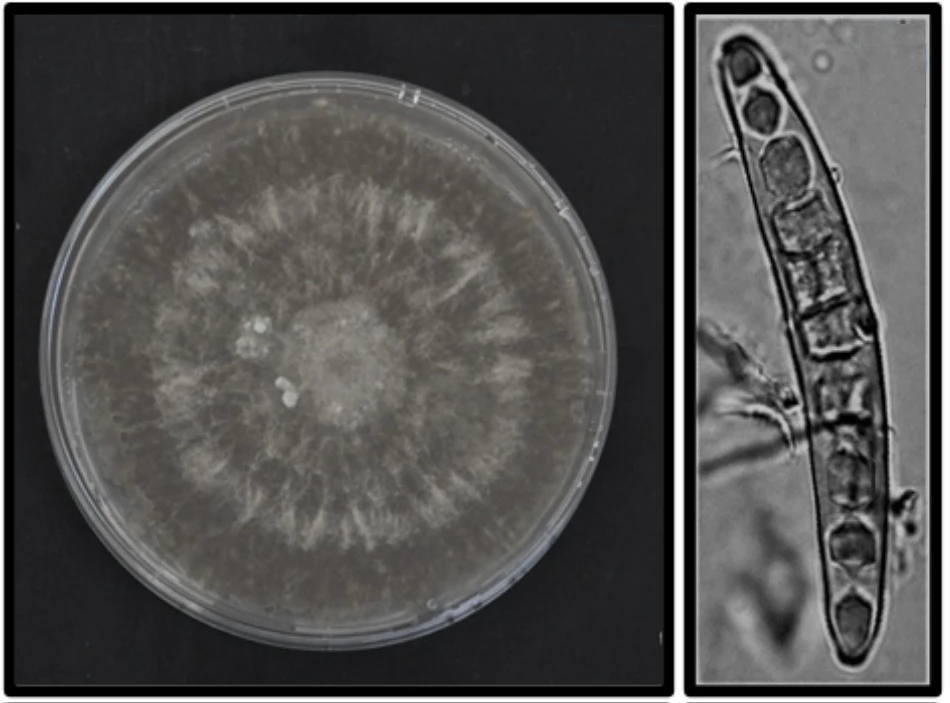
\includegraphics[width=\linewidth]{figures/real-bacteria/Exserohilum turcicum.png}
    \caption{Morphology of \textit{Exserohilum turcicum}. The left image displays a colony of Exserohilum turcicum, while the right image shows a single cell of the same species. Source: \cite{Bankole2023}.}
    \label{fig:exserohilum_turcicum}
\end{figure}

These biologically fascinating phenomena pose significant computational modeling challenges, demanding the accurate integration of both mechanical cell interactions and proliferation dynamics.

This work is directly inspired by these observations, particularly the formation of concentric rings in growing bacterial communities. These patterns represent a key manifestation of self-organization under controlled conditions, as further explored in \cite{Weady2024}. Comprehending these emergent structures necessitates robust computational models capable of capturing the dynamic interplay between individual cell mechanics, intercellular interactions, and proliferation.

\subsection{Computational Challenges}

Simulating large populations of interacting and proliferating agents, such as individual cells, presents substantial computational hurdles. Accurately representing the dynamics of active matter systems where particles interact with each other and alter the system composition through growth, demands the development of efficient algorithms. A critical challenge lies in the accurate and stable resolution of inter-particle interactions, especially in the context of collisions.

Existing constraint-based (hard) collision models, which enforce strict non-overlapping conditions via an optimization framework, offer high physical precision. However, they can incur significant computational overhead, as constraints typically require iterative, global resolution across the entire system at each simulation step. This process can become a considerable bottleneck, particularly for simulations involving vast numbers of particles or frequent collision events.

In contrast, potential-based (soft) collision models, which permit minor overlaps and employ repulsive forces to manage interactions, provide a computationally more tractable alternative by relying solely on local computations.

Despite the established trade-offs, the comparative effectiveness of hard versus soft collision models in accurately reproducing biologically relevant patterns and their computational performance within the context of proliferating cell collectives remains an underexplored area. This research aims to address this gap by systematically comparing these two modeling approaches by investigating the computational performance of both models and their ability to reproduce biologically relevant patterns.


\section{Related Work}

The simulation of collective biological behaviors, particularly the emergent patterns observed in bacterial colonies, necessitates robust computational models that accurately capture both individual cell mechanics and proliferation dynamics. Agent-based models (ABMs) are a prevalent approach, representing individual cells as discrete agents interacting within a simulated environment. A critical computational bottleneck within these ABMs is the accurate and efficient resolution of cell-cell collisions. This section reviews existing approaches to collision modeling, their computational underpinnings, and highlights a significant gap in the comparative benchmarking of these methods, particularly from a high-performance computing (HPC) perspective.

\subsection{Collision Models}

Two primary paradigms exist for handling collisions in ABMs: constraint-based (hard) collision models and potential-based (soft) collision models.


\begin{description}[style=nextline]
    \item[Constraint-Based (Hard) Collision Models]
        Constraint-based models enforce strict non-overlapping conditions between agents. This is typically achieved through optimization frameworks that resolve collisions by adjusting agent positions or velocities to satisfy geometric constraints. These methods offer high physical fidelity, ensuring that simulated agents behave as if they are truly impenetrable. \cite{Rudge2012} demonstrated a notable application of this approach for growing bacterial colonies. Their work highlighted the significant computational intensity of hard collisions, requiring methods like sparse matrix inversions for constraint resolution. They showcased the benefits of GPU acceleration for performance, achieving simulations of 30,000 cells in 30 minutes on their hardware, illustrating the substantial computational cost of such precise collision handling. This study provides a rare, explicit runtime measurement for a hard collision model, underscoring its computational demands.

    \item[Potential-Based (Soft) Collision Models]
        In contrast, potential-based (soft) collision models manage interactions by employing repulsive forces when agents approach or overlap, generally offering greater computational tractability. These models typically rely on local computations, such as calculating inter-particle forces based on proximity, making them more amenable to parallelization and large-scale simulations. \cite{Warren2019} presented a soft collision model that enabled simulations of 3D growth and complex structures, achieving impressive scalability by simulating millions of cells on multi-core CPUs. This work provides valuable insights into the performance scaling of soft collision approaches.
\end{description}

\subsection{The Benchmarking Gap: Comparative Performance of Collision Models}

While collision models have been implemented and applied to a wide range of biological systems, there is a notable lack of direct, systematic comparison focusing on their computational performance trade-offs. Many existing studies, including those that explore mechanical interactions using bacteria simulation frameworks such as \cite{Rudge2012}\cite{Weady2024}\cite{Blanchard2015}\cite{Ghosh2015}\cite{You2018}\cite{Warren2019}\cite{Khan_2024}, tend to prioritize biological insights without providing comprehensive runtime analyses or detailed HPC benchmarking across different interaction paradigms.

Specifically, the comparative effectiveness and computational cost of hard versus soft collision models within the context of proliferating cell collectives remain underexplored. A unified analysis that directly contrasts their performance characteristics (e.g., execution time, scalability, numerical stability (critical timestep), etc.) is largely absent.

This research aims to address this critical gap by systematically implementing and comparing these two collision models within a unified ABM framework, providing a much-needed computational analysis from an HPC perspective to quantify these trade-offs.

\section{Cell Mechanics}

The mechanical representation of cells significantly influences simulation outcomes. For many bacteria and fungal hyphae, a rigid rod approximation is a reasonable simplification, capturing their elongated morphology and the primary drivers of collective behavior. While real cells can exhibit some deformability, treating them as rigid bodies allows for a focus on the collective dynamics. This choice of a rigid rod geometry is well-supported by the experimental observations that inspire our work and aligns with common practices in modeling microbial collectives. The selected collision models are applied to these rigid rod entities.

\subsection{Cell Model}

For modeling the cell collectives, we use a rod model where cells are represented as rigid rods with a certain length and radius. This is a common assumption in many cell collectives models \cite{You2018}\cite{Weady2024}\cite{Blanchard2015}\cite{Warren2019}\cite{Ghosh2015} and is supported by experimental evidence, closely matching common bacteria and fungi such as \textit{E. coli} and \textit{Setosphaeria rostrata} as shown in \autoref{fig:exserohilum_turcicum}.


Each bacterium is represented by a spherocylinder with initial length $l=1$ and diameter $d=0.5$. At the scale of typical bacteria, the system can be represented by an overdamped dynamics, because their Reynolds number is extremely small (Re $\ll 1$), so viscous drag stops them from coasting almost instantaneously \cite{datta2024lifelowreynoldsnumber}. The resulting dynamics is then described by the overdamped Langevin equation:

\begin{equation}
    \frac{d \mathbf{x}_i}{dt} = \frac{1}{\zeta l_i} \sum_j \mathbf{F}_{ij}, \quad \frac{d \mathbf{\omega}_i}{dt} = \frac{12}{\zeta l_i^3} \sum_j (\mathbf{r}_{ij} \times \mathbf{F}_{ij})
\end{equation}
\label{eq:overdamped_langevin}

where $\mathbf{x}_i$ is the position of the cell, $\mathbf{\omega}_i$ is the angular velocity of the cell, $\mathbf{F}_{ij}$ is the force acting on the cell from the $j$-th cell. $\zeta$ is a constant drag coefficient representing the friction of the cell in the fluid, $\mathbf{r}_{ij}$ is the point of contact between the two cells relative to the center of the $i$-th cell.

\autoref{fig:spherocylinder_model} illustrates the spherocylinder model and the relevant forces and torques acting on the cells during a collision.

\begin{figure}[H]
    \centering


    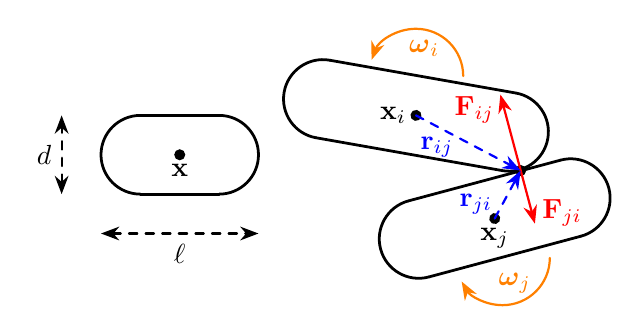
\begin{tikzpicture}[line cap=round,line join=round,>=Stealth]

        % --- Variables ---
        \coordinate (xi) at (0,0);
        \coordinate (xj) at (1,-1.31);

        \coordinate (x) at (-3,-0.5);
        \def\R{0.5}

        \drawSpherocyl{xi}{-10}{1.2}{\R}
        \drawSpherocyl{xj}{15}{1}{\R}

        \coordinate (contact) at  (1.33,-0.7);

        % Collision point
        \fill[black] (contact) circle (2pt) node[above right] {};

        % Force vector
        \draw[->,thick,red] (contact) -- ++(-0.258,0.965) node[pos=0.8,left] {$\mathbf{F}_{ij}$};

        % Torque lever arm
        \draw[->,thick,blue,dashed] (xi) -- (contact) node[pos=0.2,below] {$\mathbf{r}_{ij}$};

        % Force vector
        \draw[->,thick,red] (contact) -- ++($0.7*(0.258,-0.965)$) node[pos=0.8,right] {$\mathbf{F}_{ji}$};

        % Torque lever arm
        \draw[->,thick,blue,dashed] (xj) -- (contact) node[pos=0.3,left] {$\mathbf{r}_{ji}$};



        % label at xi
        \node at (xi) [left] {$\mathbf{x}_i$};
        % label at xj
        \node at (xj) [below] {$\mathbf{x}_j$};


        \drawSpherocyl{x}{0}{0.5}{\R}

        % label at x
        \node at (x) [below] {$\mathbf{x}$};

        \draw[<->,thick,dashed] ($(x) + (-0.5-\R,-1)$) -- ($(x) + (0.5+\R,-1)$) node[midway,below] {$\ell$};

        \draw[<->,thick,dashed] ($(x) + (-0.5-\R-\R,-\R)$) -- ($(x) + (-0.5-\R-\R,\R)$) node[midway,left] {$d$};


        % Resulting rotation around xi
        \draw[->,thick,orange]
        ($(xi)+(0.6,0.5)$) arc[start angle=0,end angle=160,radius=0.6]
        node[midway, below] {$\boldsymbol{\omega}_i$};

        % Resulting rotation around xj
        \draw[->,thick,orange]
        ($(xj)+(0.7,-0.5)$) arc[start angle=0,end angle=-150,radius=0.6]
        node[midway, above] {$\boldsymbol{\omega}_j$};

    \end{tikzpicture}
    \caption{2D Schematic of the spherocylinder cell model. Each cell has length $\ell$ and diameter $d$. Collisions generate contact forces $\mathbf{F}_{ij}$ (red) and torque via the lever arm $\mathbf{r}_{ij}$ (dashed blue). The resulting translations are proportional to the force vectors, and the change in orientation follows from the cross product $\mathbf{r}_{ij} \times \mathbf{F}_{ij}$, indicated here in orange.
    }
    \label{fig:spherocylinder_model}

\end{figure}


Bacteria cells grow along their main axis using the following model in accordance with \cite{Weady2024}:

\begin{equation}
    \dot{{\ell}} =  \frac{{\ell}}{\tau} e^{\lambda \boldsymbol{\sigma}}
\end{equation}


where $\tau$ is a time scale, $\sigma$ is the compressive stress along the main axis of the cell, and $\lambda$ is a stress sensitivity parameter which will later be used to control the growth rate and the macroscopic pattern formation of the colony.

Once a bacteria cell reaches a certain length ($\ell_0 = 2\ell_0$), it will divide into two new cells. To avoid synchronization effects, we adapt the model from \cite{Weady2024} and slighly change the length of the daughter cells randomly between $\ell_0 \cdot 0.98$ and $\ell_0 \cdot 1.02$ as proposed in \cite{Khan_2024}.

\newpage
\subsection{Colony Representation}

For the implementation we closely follow the approach of Weady et al. \cite{Weady2024} described in the supplementary material where the whole bacteria colony gets represented in a single global vector $\mathbfcal{C} = [\dots, x_n^T, w_n^T, \dots]^T \in \mathbb{R}^{7N}$ where $N$ is the number of cells in the colony. Each particle is thus represented by a 7-dimensional vector consisting of a position vector $x_n \in \mathbb{R}^3$ and a unit quaternion $q_n \in \mathbb{R}^4$ representing the cell's orientation. The length vector $\boldsymbol{\ell} = [\dots, \ell_n, \dots]^T \in \mathbb{R}^{N}$ is stored seperately.

\subsection{Colony Dynamics}

We determine the resulting translational and angular velocity for particles in the colony by using the force-velocity relation $\mathbfcal{U} = \mathbfcal{M} \mathbfcal{F}$, where $\mathbfcal{F}$ is the generalized force vector consisting of both force and torque components for the whole colony and $\mathbfcal{M}$ is the mobility matrix. $\mathbfcal{U}$ and $\mathbfcal{F}$ are also stacked collumn vectors, where $\mathbfcal{F} = [\dots, f_n^T, t_n^T, \dots]^T \in \mathbb{R}^{6}$ represents the force and torque for the $n$-th cell, $\mathbfcal{M} = \text{diag}([\dots, \frac{1}{l_n}, \frac{12}{l_n^3}, \dots]) \in \mathbb{R}^{6 \times 6}$ is a diagonal matrix consisting of the inverse of the cell's linear and angular mobility on the diagonal and $\mathbfcal{U} = [\dots, u_n^T, \omega_n^T, \dots]^T \in \mathbb{R}^{6}$ represents the resulting translational and angular velocity for the $n$-th cell.

Combined with a map $\mathbfcal{G}$ mapping cartesian translational and angular velocities from $\mathbb{R}^{6N}$ to the corresponding change in position and quaternion in $\mathbb{R}^{7N}$, described in \cite{Weady2024}, we can express the resulting colony state after applying force and torque $\mathbfcal{F}$ for an euler timestep $\Delta t$ as:

\begin{equation}
    \mathbfcal{C}^{k+1}  = \mathbfcal{C}^k + \Delta t \, \mathbfcal{G}^k\mathbfcal{U} = \mathbfcal{C}_k + \Delta t \, \mathbfcal{G}\mathbfcal{M} \mathbfcal{F}
\end{equation}
\label{eq:colony_update}



Now we can define the specific implementations of hard and soft collision models by specifying how the force vector $\mathbfcal{F}$ is computed in each case.

\newpage

\subsection{Soft Collision Model}

For the soft collision model, we consider a potential-based approach inspired by \cite{Warren2019} and \cite{You2018} where overlapping cells exert repelling forces on each other based on a predefined potential function. In particular, we implement a Hertzian potential, which provides a smooth force response as particles approach each other.

We use the following Model for the elastic force between two overlapping particles:

\begin{equation}
    \mathbf{F}_{elastic} =k_{cc} \sqrt{d_0} \delta^{1.5} \hat{\mathbf{n}}
\end{equation}
\label{eq:hertzian_contact_model}

where $\delta$ is the overlap distance between the particles, $k_{cc}$ is the elastic constant, and $\hat{\mathbf{n}}$ is the normal vector at the point of contact. \autoref{fig:hertzian_contact_model} illustrates the force response of this model as a function of overlap distance.

Using equation \autoref{eq:overdamped_langevin} we can then express the total force and torque of each cell. From this we can construct the full force vector $\mathbfcal{F}$ for the whole colony and use \autoref{eq:colony_update} to update the colony state.

Inspired from  \cite{You2018} we set $k_{cc} = \frac{Y}{\zeta} = \frac{4 MPa}{200 Pa h} = 20000 \frac{1}{h}$ and use a typical time step $\Delta t \approx 10^{-5} h$ \cite{Khan_2024}\cite{You2018}\cite{Blanchard2015}.


\begin{figure}[H]
    \centering
    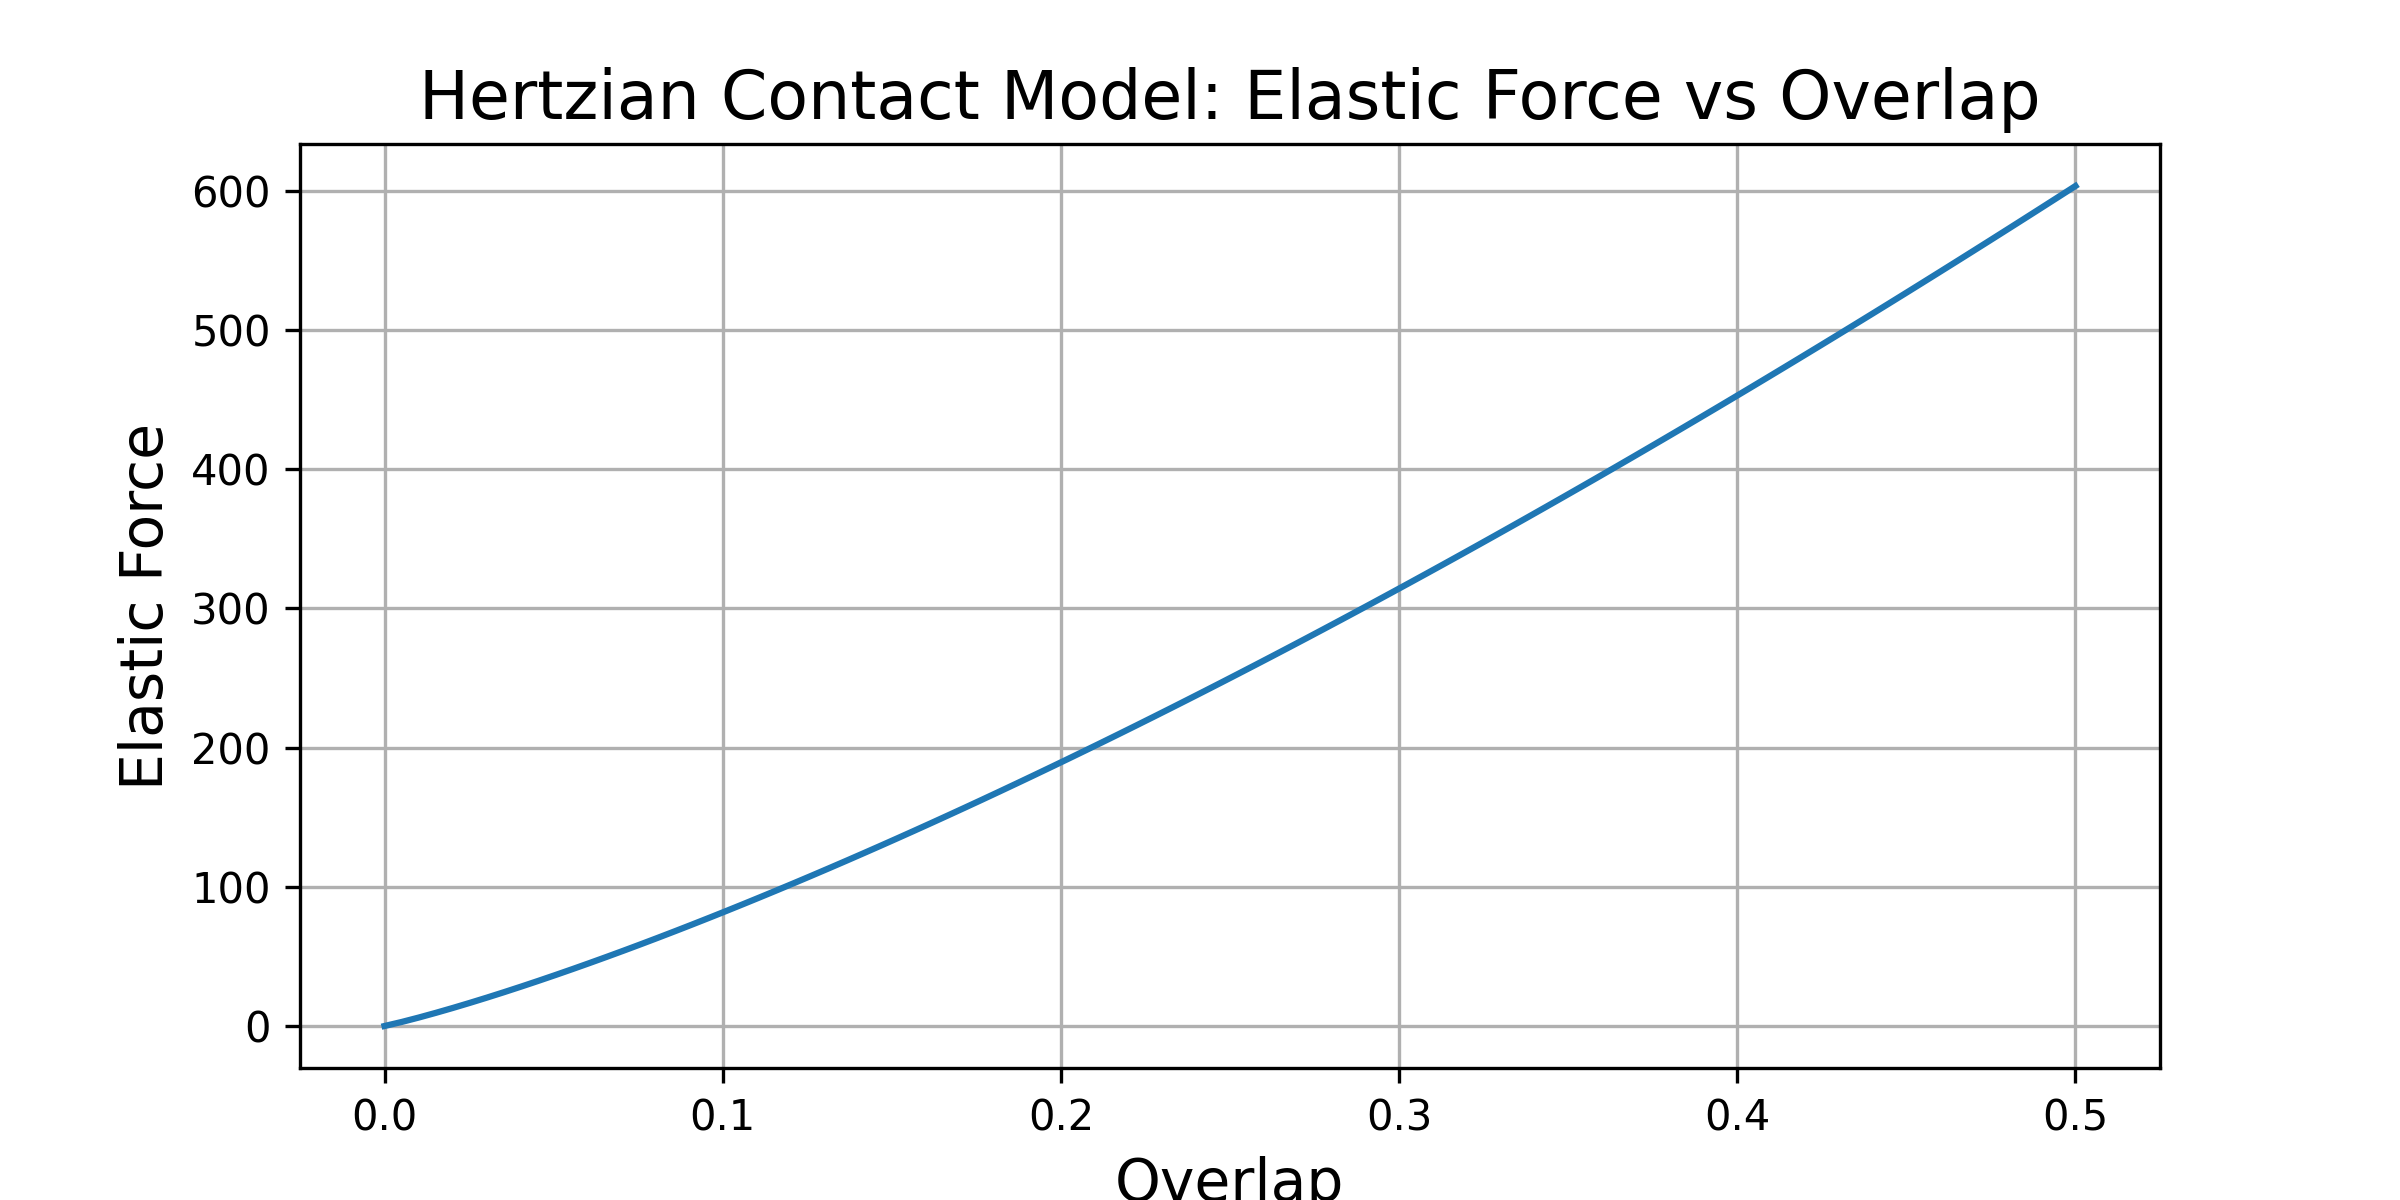
\includegraphics[width=\linewidth]{figures/hertzian_contact_model.png}
    \caption{Elastic force as a function of overlap distance for the implemented Hertzian contact model with $k=2000$ and $\alpha=0.5$.}
    \label{fig:hertzian_contact_model}
\end{figure}

\newpage
\subsection{Hard Collision Model}


For the hard collision model, we want to enforce non-overlapping constraints between cells using a constraint-based approach. Therefore we create a constraint $\alpha$ for each pair of nearby cells consisting of the two closest points $\mathbf{y}_n$ and $\mathbf{y}_m$ on the surfaces of the two particles.

Contrary to \autoref{eq:hertzian_contact_model} where the force magnitude is computed using a function based on the overlap distance, we define the force and torque contributions from each constraint directly in terms of the yet unknown force magnitude $\gamma_\alpha$ needed to satisfy the non-overlapping condition.

\begin{equation}
    \mathbf{F}_\alpha^n = \hat{\mathbf{n}}_\alpha ^n \gamma_\alpha
\end{equation}
\label{eq:constraint_force}

To simplify the notation we combine all lagrange multplieres $\gamma_\alpha$ into a single vector $\boldsymbol{\gamma} = [\dots, \gamma_\alpha, \dots]^T \in \mathbb{R}^{C}$ where $C$ is the total number of constraints in the system.

From this we can again calculate the total forces and torques acting on the colony by \autoref{eq:overdamped_langevin}. The resulting force vector $\mathbfcal{F}$ now depends linearly on the unknown multipliers $\boldsymbol{\gamma}$ and will from now on be denoted as $\mathbfcal{F}(\boldsymbol{\gamma}) = \mathbfcal{D}\boldsymbol{\gamma}$ where $\mathbfcal{D} \in \mathbb{R}^{6N \times C}$ is a matrix consisting of the normal vectors $\hat{\mathbf{n}}_\alpha$ and torque arms $\mathbf{y}_n \times \hat{\mathbf{n}}_\alpha$ for each constraint $\alpha$ and particle $n$. The multiplication $\mathbfcal{D}\boldsymbol{\gamma}$ thus computes the total force and torque on each particle from all constraints as described in \autoref{eq:constraint_force}.

\subsection{Constraint Resolution}

Moreover we define $\mathbf{\Phi}^k = [\dots, \Phi_\alpha, \dots]^T \in \mathbb{R}^{C}$ as the vector of signed seperation distances for the respective pair of particles at the current time step $k$.

\subsubsection{Constraint Conditions}

When solving for the Lagrange multipliers $\boldsymbol{\gamma}$, we are only interested in \emph{repelling} forces, i.e.\ forces that separate overlapping particles.
Since attractive forces are not physically meaningful, the multipliers must be nonnegative (see~\autoref{eq:gamma}).
Furthermore, after the update step the particle configuration must be feasible, meaning that no overlaps remain (see~\autoref{eq:phi}).

The multipliers act during the current step in order to enforce this feasibility in the \emph{next} configuration.
For this reason the complementarity condition is formulated with $\Phi^{k+1}$: if a constraint is inactive after the update ($\Phi_\alpha^{k+1} > 0$), then the corresponding multiplier must vanish ($\gamma_\alpha = 0$), whereas if a multiplier is nonzero ($\gamma_\alpha > 0$), then the constraint must be active at the updated configuration ($\Phi_\alpha^{k+1} = 0$).
This is expressed by the \emph{complementarity condition} (see~\autoref{eq:comp}).

Altogether, the contact problem can be written as
\begin{align}
    \text{Positivity of multipliers:} \qquad & \boldsymbol{\gamma} \geq 0, \label{eq:gamma}                   \\
    \text{Non-overlap condition:} \qquad     & \mathbf{\Phi}^{k+1} \geq 0, \label{eq:phi}                     \\
    \text{Complementarity condition:} \qquad & \boldsymbol{\gamma} \perp \mathbf{\Phi}^{k+1}, \label{eq:comp}
\end{align}
which is often abbreviated as $\mathbf{0} \leq \boldsymbol{\gamma} \perp \mathbf{\Phi}^{k+1} \geq \mathbf{0}$.


The combined update rule in \autoref{eq:colony_update} and the constraint conditions above can be combined into a single system of equations to solve for the unknown Lagrange multipliers $\boldsymbol{\gamma}$:

\begin{align}
    \mathbfcal{C}^{k+1} & = \mathbfcal{C}^k + \Delta t \, \mathbfcal{G}\mathbfcal{F}(\boldsymbol{\gamma}) = \mathbfcal{C}^k + \Delta t \, \mathbfcal{G}\mathbfcal{M} \mathbfcal{D} \boldsymbol{\gamma} \\
    \text{s.t.} 0       & \leq \boldsymbol{\gamma} \perp \mathbf{\Phi}^{k+1} \geq 0
\end{align}


As $\mathbf{\Phi}^{k+1}$ is difficult to express in closed form as it depends on the updated colony state $\mathbfcal{C}^{k+1}$ which itself depends on $\boldsymbol{\gamma}$, Weady et al. \cite{Weady2024} approximate it using a first-order Taylor expansion around the current state $\mathbfcal{C}^k$:

\begin{align}
    \mathbf{\Phi}^{k+1} & \approx \mathbf{\Phi}^k + \Delta t (\mathbfcal{D}^T \dot{\mathbfcal{C}^k} - \mathbfcal{L}^T \dot{\boldsymbol{\ell}^k})                                   \\
                        & = \mathbf{\Phi}^k + \Delta t (\mathbfcal{D}^T \mathbfcal{G} \mathbfcal{M} \mathbfcal{D} \boldsymbol{\gamma} - \mathbfcal{L}^T \dot{\boldsymbol{\ell}^k})
\end{align}.

It is obvious from the equation that the change in signed seperation distances $\mathbf{\Phi}$ depends on two factors: the motion of the cells and their growth. The term $\dot{\mathbfcal{C}^k} = \mathbfcal{G} \mathbfcal{M} \mathbfcal{D} \boldsymbol{\gamma}$ describes how the colony state changes due to the forces exerted by the constraints, while $\dot{\boldsymbol{\ell}^k}$ describes how the lengths of the cells change. The matrix $\mathbfcal{L}$ consists of the stre

where $\mathbfcal{L} \in \mathbb{R}^{N \times C}$ consists of the normalized stress values acting on a pair of cells for each constraint $\alpha$.

The resulting system of equations to solve for $\boldsymbol{\gamma}$ is thus

\begin{align}
    \mathbfcal{C}^{k+1} & = \mathbfcal{C}^k + \Delta t \, \mathbfcal{G}\mathbfcal{M} \mathbfcal{D} \boldsymbol{\gamma}                                                                                                 \\
    \text{s.t.} 0       & \leq \boldsymbol{\gamma} \perp \mathbf{\Phi}^k + \Delta t (\mathbfcal{D}^T \mathbfcal{G} \mathbfcal{M} \mathbfcal{D} \boldsymbol{\gamma} - \mathbfcal{L}^T \dot{\boldsymbol{\ell}^k}) \geq 0
\end{align}

which is a well-known form of a Linear Complementarity Problem (LCP).The missing Lagrange multipliers $\boldsymbol{\gamma}$ can be solved for using various numerical methods such as the the BBPGD algorithm described in \cite{Weady2024} and can then be used to compute the resulting force vector $\mathbfcal{F}(\boldsymbol{\gamma})$ and update the colony state using \autoref{eq:colony_update}.

Weady et al. \cite{Weady2024} improve this basic scheme by introducing a recursive approach to resolve violations of the non-overlapping condition, which can occur due to the first-order approximation of $\mathbf{\Phi}^{k+1}$. We will not go into further detail here, but refer to their supplementary material for a comprehensive description of the full algorithm.

\subsection{Stress Calculation}
To compute the stress $\boldsymbol{\sigma}$ acting on each cell, we follow the approach of \cite{Weady2024} and sum over all compressive forces projected onto the cell’s main axis. For cell $n$ this gives

\begin{equation}
    \boldsymbol{\sigma}_n = \sum_{\alpha \in A_n}
    \frac{1}{2} \left |\hat{\mathbf{t}}_n \cdot \hat{\mathbf{n}}_\alpha \right | f_\alpha,
\end{equation}

where $\hat{\mathbf{t}}_n$ is the unit vector perpendicular to the cell’s axis, $\hat{\mathbf{n}}_\alpha$ the contact normal of constraint $\alpha$, and $A_n$ the set of all constraints acting on cell $n$. The contact force magnitude $f_\alpha$ depends on the collision model:

\begin{description}
    \item[Hard model:]  $f_\alpha = \gamma_\alpha$, the Lagrange multiplier associated with constraint $\alpha$.
    \item[Soft model:] $f_\alpha = k_{cc} \sqrt{d_0}\,\delta^{1.5}$, given by the Hertzian contact law (see \autoref{eq:hertzian_contact_model}).
\end{description}



\newpage

\section{Implementation and Results}

All the simulations presented in this paper were conducted using a framework for simulating proliferating cell collectives. The framework implements both the hard and soft collision models and closely followes the mathematical formulations presented in the previous section. To achieve a good performance we leverage PETSc \cite{petsc-web-page} for efficient parallel processing and sparse matrix operations, enabling scalability. Our primary objective in this section is to compare the performance characteristics and pattern formation capabilities of these two models, with a particular focus on identifying the computational advantages of the soft collision approach. The simulation code is publicly available at {\color{blue}\url{https://github.com/manuellerchner/MicrobeGrowthSim-IDP}}.








\subsection{Simulation Framework}
\begin{itemize}
    \item Implementation details
    \item Data structures
    \item Performance optimization
\end{itemize}

\newpage

\subsection{Pattern Formation Analysis}

\subsubsection{Concentric Ring Patterns}

We first validate our implementations by reproducing the concentric ring patterns observed under stress-sensitive growth conditions, as documented in \cite{Weady2024}. Simulations were conducted for $\lambda = 10^{-1}, 10^{-2}, 10^{-3}$ using both hard and soft collision models. As presented in \autoref{fig:pattern_formation}, both models successfully generate qualitatively similar emergent ring structures. This indicates that the soft collision model, despite its simpler underlying mechanics, can adequately capture the essential dynamics leading to these macroscopic patterns, suggesting it is a viable and potentially more efficient alternative for pattern formation studies.


Notably, the soft model also produces the expected concentric ring patterns, while using a drastically simplified approach to handling collision resolution.

This suggests that, for the purpose of reproducing such patterns, the soft collision model is a viable alternative to the more complex hard collision approach.

\begin{figure*}[p]
    \centering

    % Lambda = 10^-1 comparison
    \begin{subfigure}[b]{\textwidth}
        \centering
        \caption{Growth Comparison $\lambda=10^{-1}$}
        \begin{tabular}{r M{\subfigwidth} M{\subfigwidth} M{\subfigwidth} M{\subfigwidth}}
            \growthcomparisonrow{Hard}{1e-1}{0400}{0800}{1200}{1800}
            \growthcomparisonrow{Soft}{1e-1}{0400}{0800}{1200}{1800}
        \end{tabular}
    \end{subfigure}

    % % Lambda = 10^-2 comparison
    \begin{subfigure}[b]{\textwidth}
        \centering
        \caption{Growth Comparison $\lambda=10^{-2}$}
        \begin{tabular}{r M{\subfigwidth} M{\subfigwidth} M{\subfigwidth} M{\subfigwidth}}
            \growthcomparisonrow{Hard}{1e-2}{0400}{0700}{0900}{1100}
            \growthcomparisonrow{Soft}{1e-2}{0400}{0700}{0900}{1100}
        \end{tabular}
    \end{subfigure}

    % Lambda = 10^-3 comparison
    \begin{subfigure}[b]{\textwidth}
        \centering
        \caption{Growth Comparison $\lambda=10^{-3}$}
        \begin{tabular}{r M{\subfigwidth} M{\subfigwidth} M{\subfigwidth} M{\subfigwidth}}
            \growthcomparisonrow{Hard}{1e-3}{0400}{0600}{0800}{1000}
            \growthcomparisonrow{Soft}{1e-3}{0400}{0600}{0800}{1000}
        \end{tabular}
    \end{subfigure}


    \caption{Pattern formation under stress-sensitive growth at equally spaced time points. Each row shows the evolution for a different value of $\lambda$ for both hard and soft collision models up to a maximum colony radius of 50. The color indicates the length of the cells ranging from 1 (dark green) to 2 (light green). Clear concentric ring pattern are visible for $\lambda \in \{10^{-2}, 10^{-3}\}$.}
    \label{fig:pattern_formation}
\end{figure*}



\subsubsection{Microdommain formation}

\cite{You2018}


\newpage

\subsection{Quantitative Comparison}

For a more quantitative comparison, we analyze the following metrics: \textit{radial distribution of stress}, \textit{radial distribution of packing fraction} and \textit{maximum overlap}.

Figures~\ref{figure:radial_distribution_stress}--\ref{figure:max_overlap_simulation} illustrate these results in detail. Those figures confirm that altough certain quantities, such as the packing fraction, and thus the maximum overlap, are different between the two models (See \autoref{fig:dense_packing_comparison}), the overall macroscopic behavior is similar as previously anayzed in \autoref{fig:pattern_formation}.


\begin{figure}[h]
    \centering
    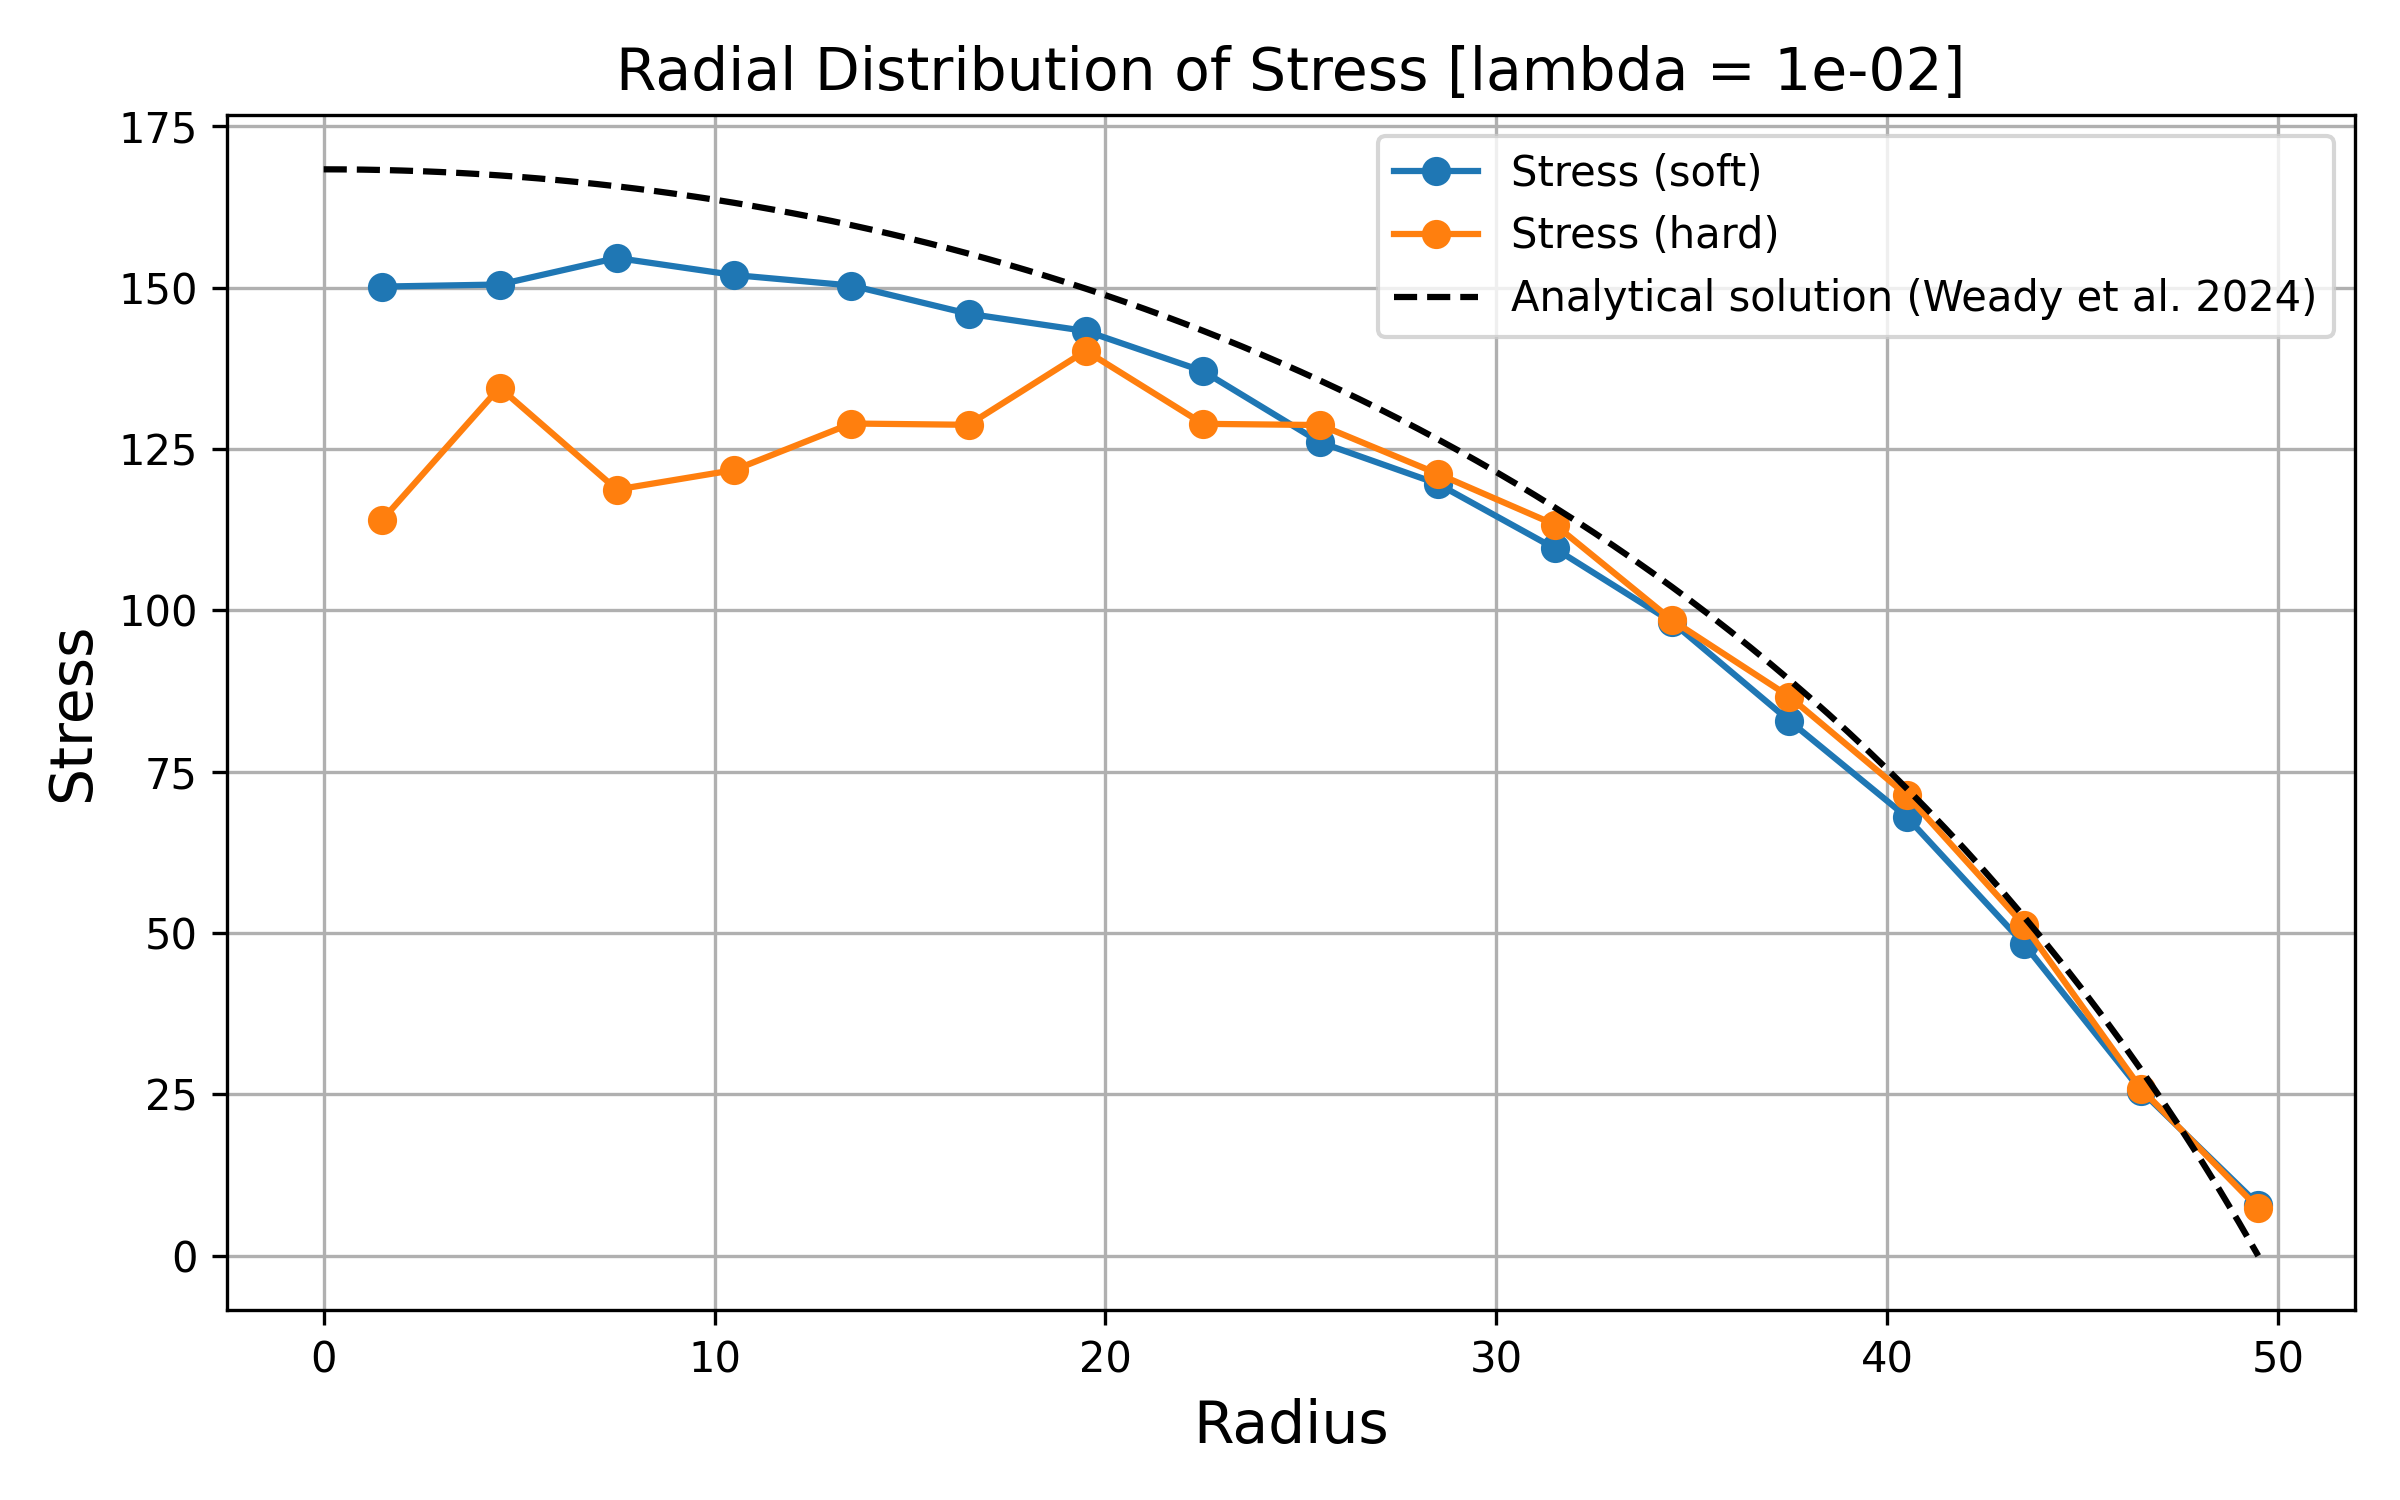
\includegraphics[width=\linewidth]{figures/comparisons/radial_distribution_stress.png}
    \caption{Comparison of the radial distribution of the stress for the hard and soft collision models. Both models reproduce the expected stress distribution analytically derived in \cite{Weady2024}.}
    \label{figure:radial_distribution_stress}
\end{figure}

\begin{figure}[h]
    \centering
    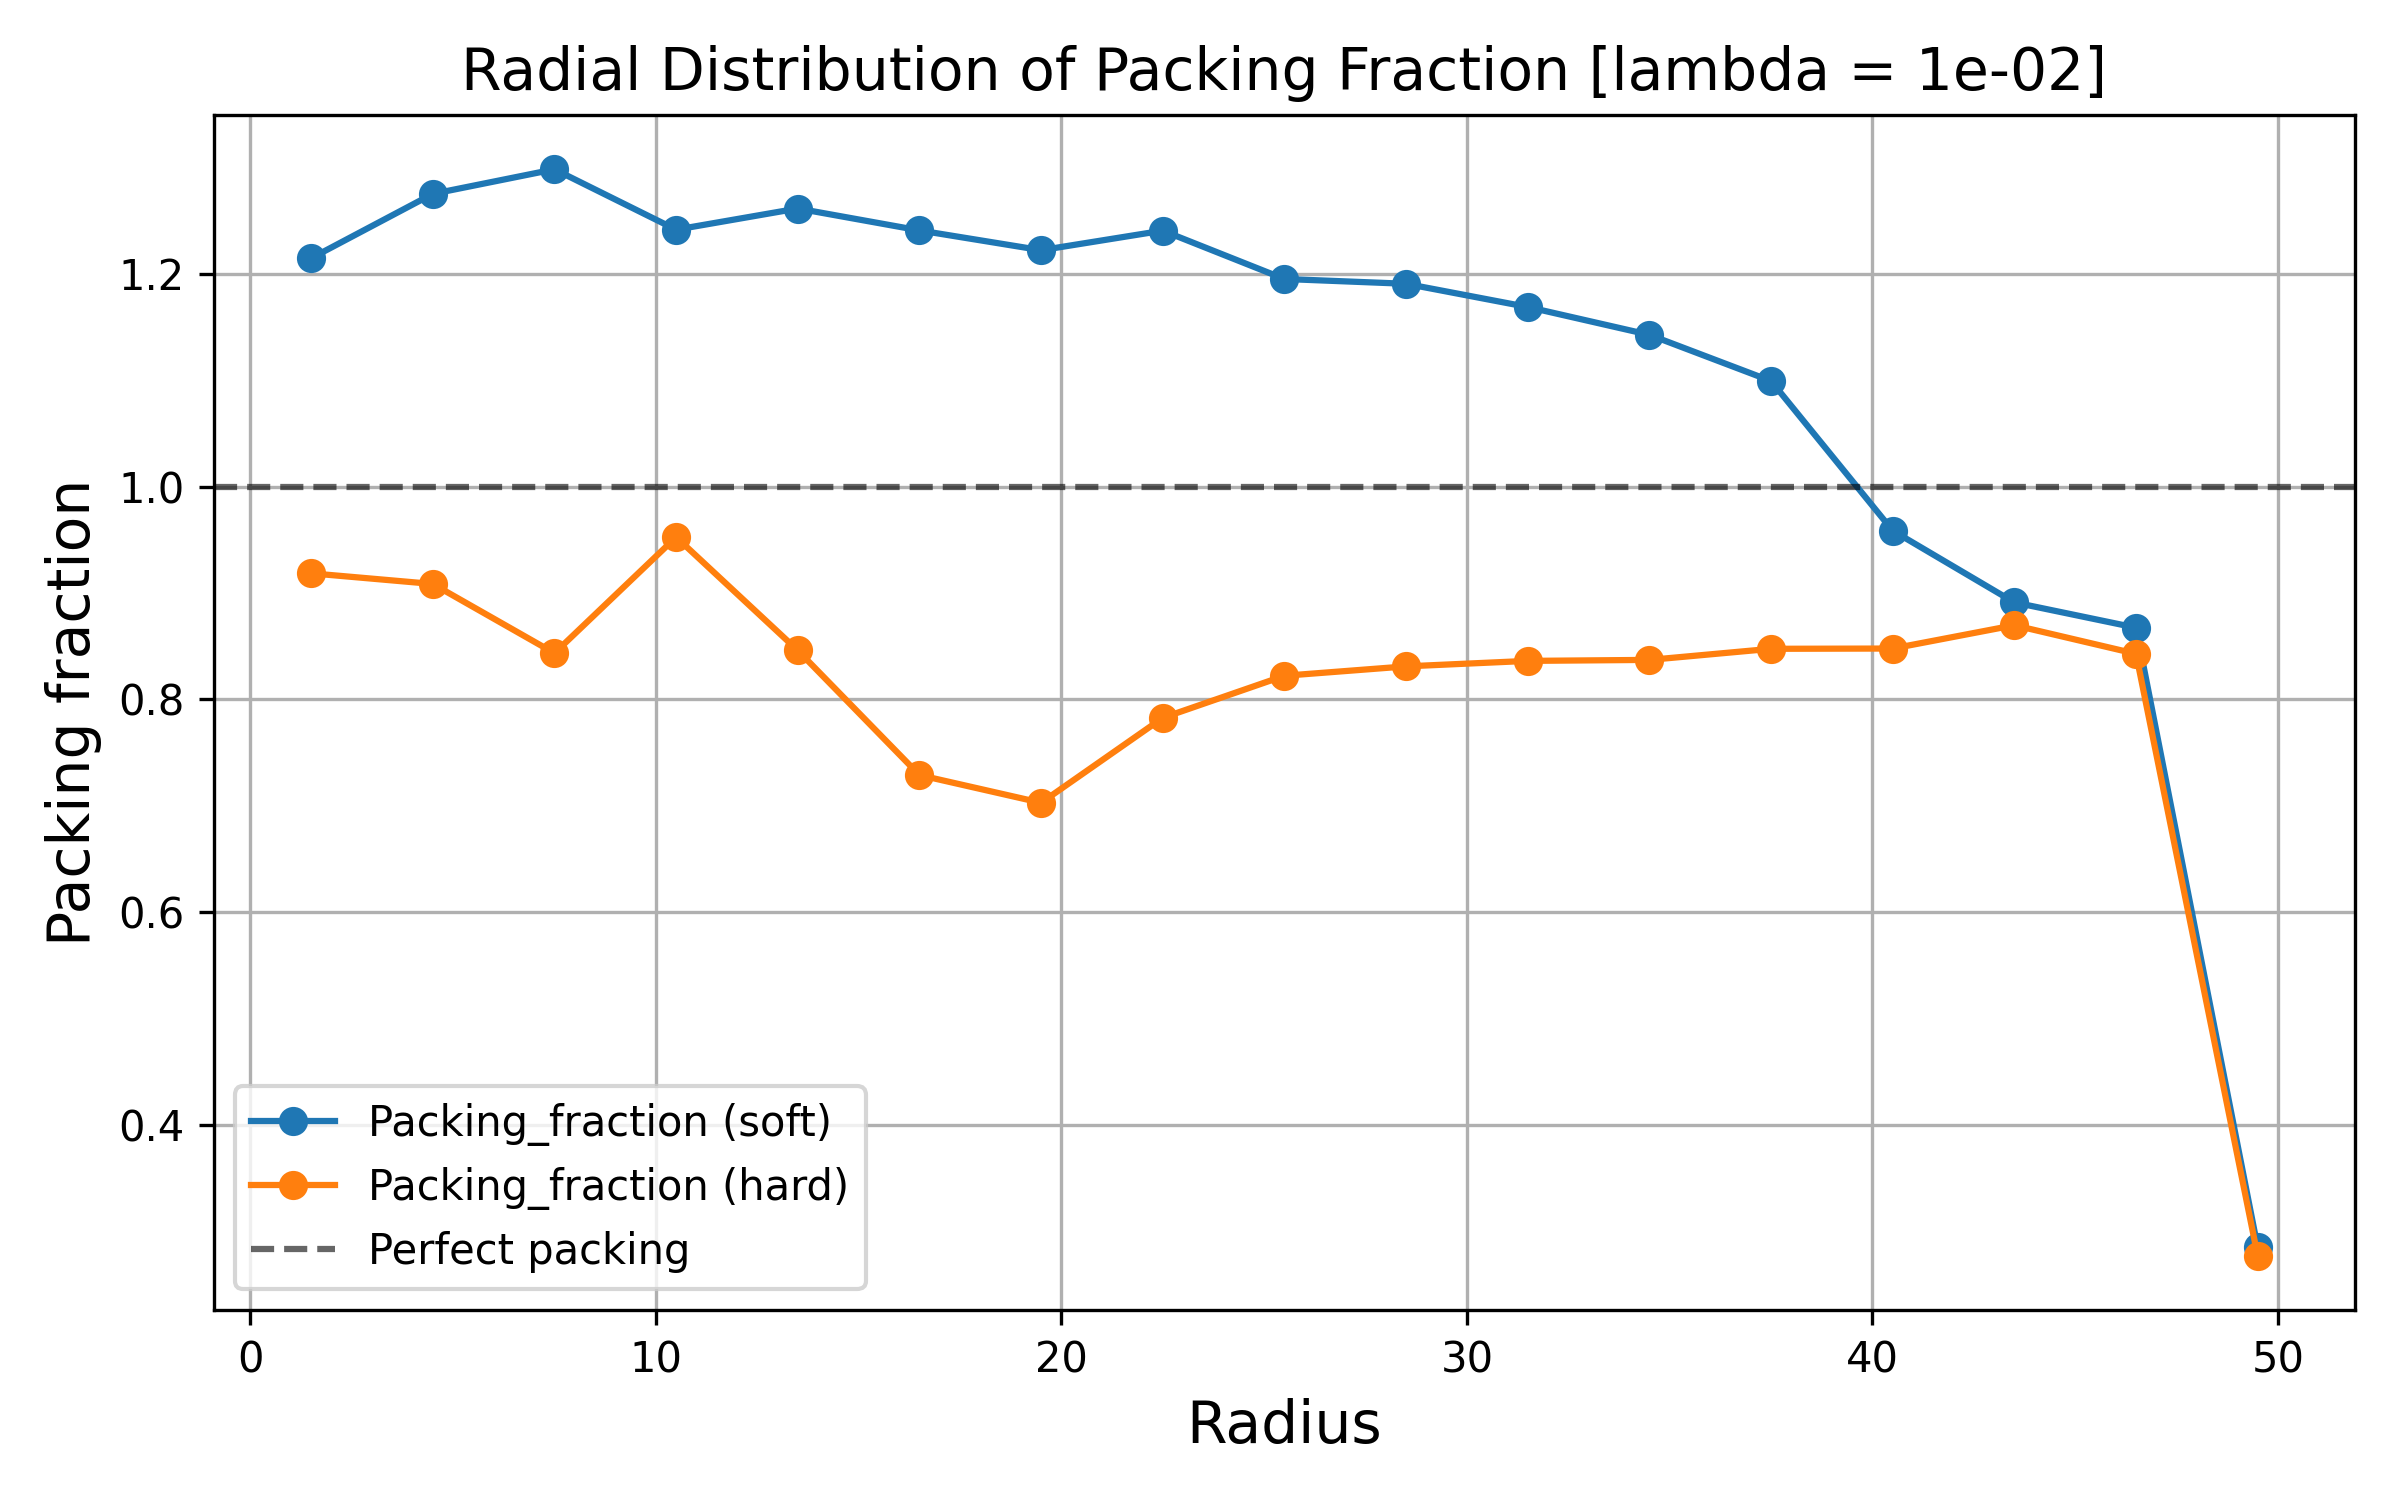
\includegraphics[width=\linewidth]{figures/comparisons/radial_distribution_packing_fraction.png}
    \caption{Comparison of the radial distribution of the packing fraction for the hard and soft collision models. As expected, particles in the soft model experience some overcrowding at the center of the colony, but the overall distribution is similar to the hard model.}
    \label{figure:radial_distribution_packing_fraction}
\end{figure}

\begin{figure}[h]
    \centering
    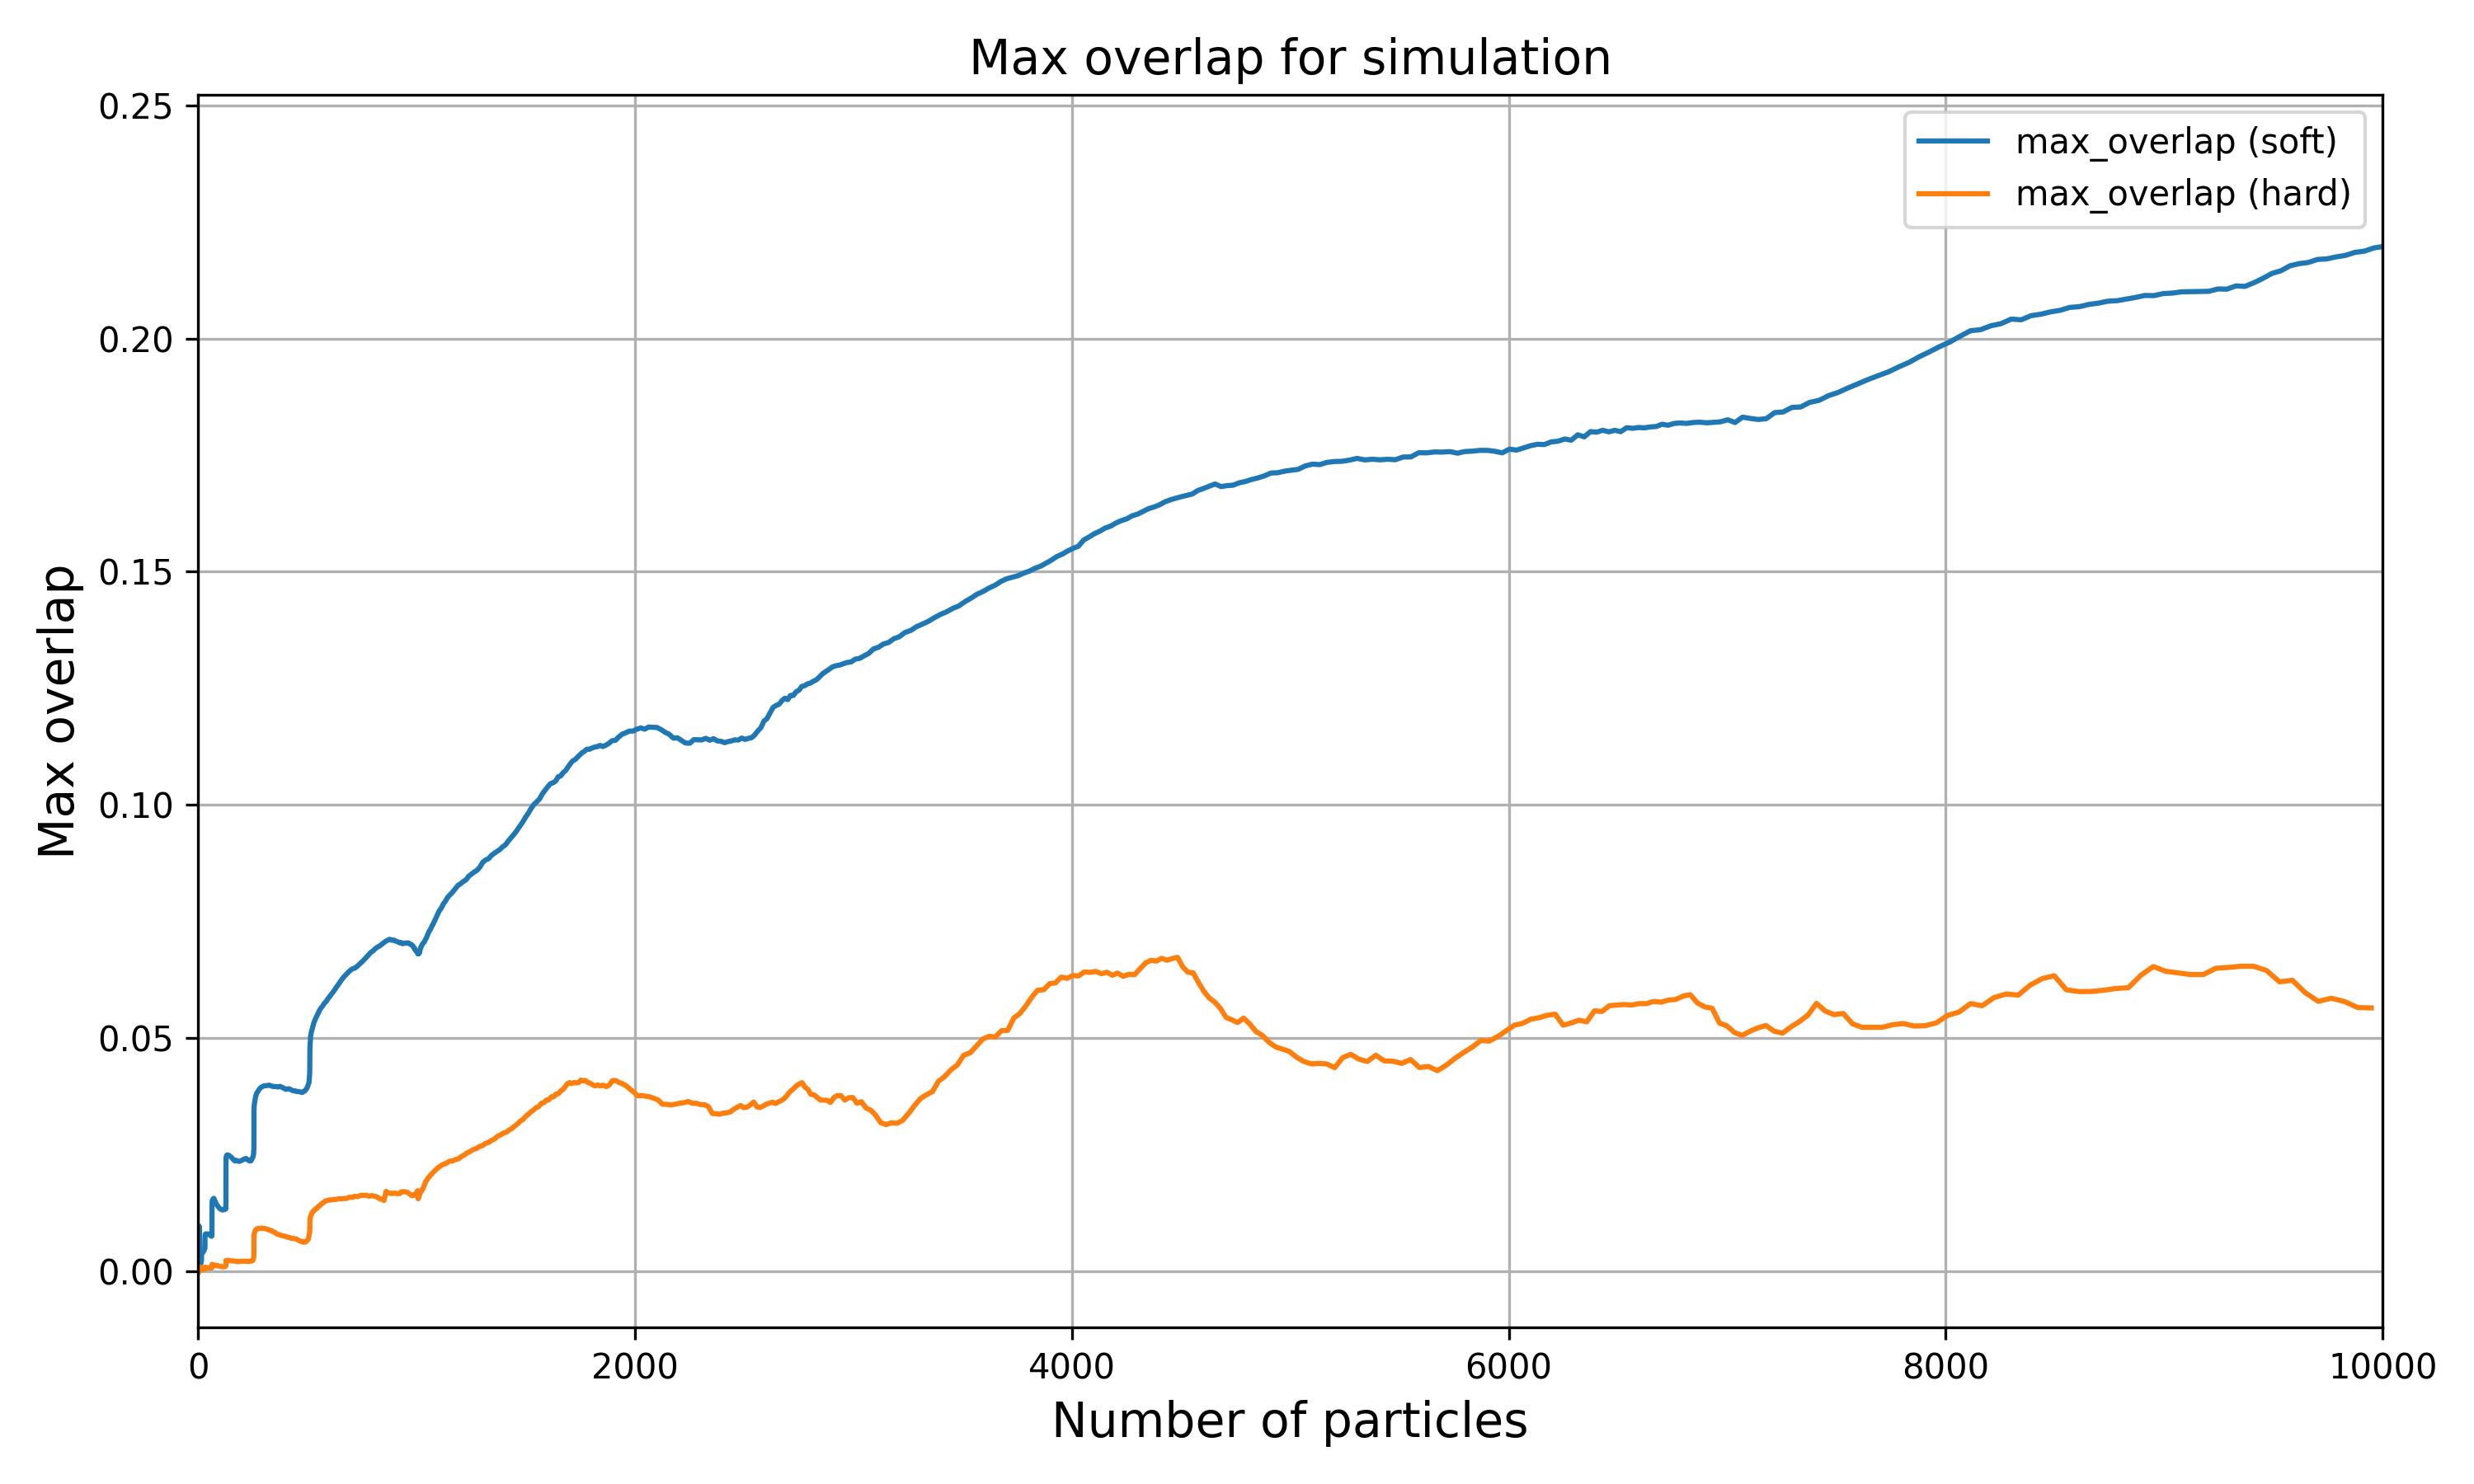
\includegraphics[width=\linewidth]{figures/comparisons/max_overlap_simulation.png}
    \caption{Comparison of the maximum overlap for the hard and soft collision models. The maximum overlap between particles in the soft model increases over time, while it is kept close to a constant value (determined by the tolerance parameter) in the hard model.}
    \label{figure:max_overlap_simulation}
\end{figure}


\begin{figure}
    \centering
    \begin{subfigure}[b]{0.49\columnwidth}
        \centering
        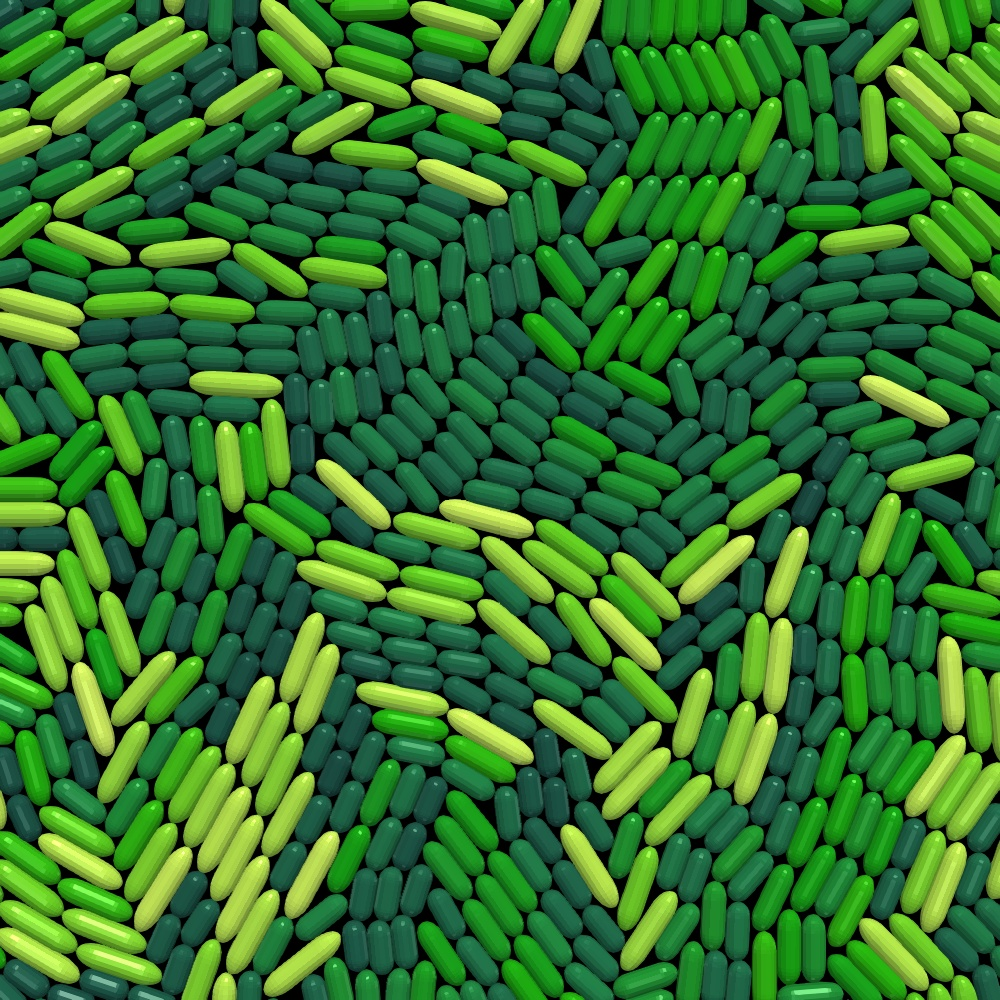
\includegraphics[width=\linewidth]{figures/comparisons/packing_hard.jpeg}
        \caption{Close up of the particle packing for the hard model.}
        \label{fig:sensor3}
    \end{subfigure}
    \begin{subfigure}[b]{0.49\columnwidth}
        \centering
        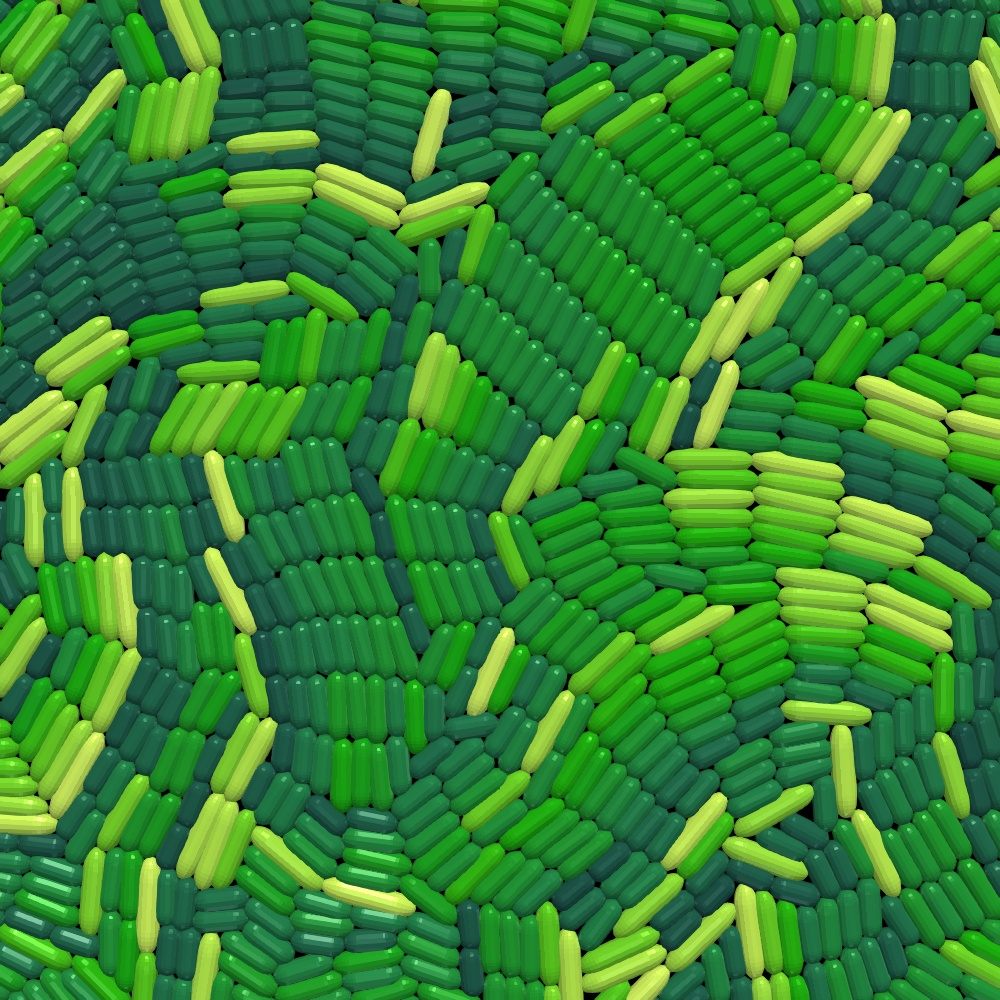
\includegraphics[width=\linewidth]{figures/comparisons/packing_soft.jpeg}
        \caption{Close up of the particle packing for the soft model.}
        \label{fig:tiger}
    \end{subfigure}
    \caption{Close up of the particle packing for the hard and soft collision models. The soft model exhibits denser packing with slightly overlapping particles.} \label{fig:dense_packing_comparison}
\end{figure}



\newpage

\section{Computational Performance}

While both models reproduce the observed patterns, our preliminary analysis suggests significant performance differences. The hard collision model's requirement to solve an LCP at each time step introduces a computational bottleneck, potentially limiting its scalability for very large systems or long simulation times. In contrast, the direct force calculation in the soft collision model is inherently less complex per interaction but typical needs to be computed using a finder time step to avoid instabilities.


Moreover solving a LCP requires global information about the system, as it is essentially optimizing a global system of constraints. This can lead to increased communication overhead in parallel implementations, as all processors take part in an iterative solver and are required to share information about all particles in the system during each optimization step.


In contrast, the soft collision model only requires local information about neighboring particles to compute forces, and can be efficiencyly computed using common molecular dynamics techniques such as cell lists or Verlet lists (See \cite{Gratl2019}). This locality greatly reduces the amount of inter-processor communication needed in a parallel implementation, as each processor can largely operate independently on its own subset of particles, only needing to occasionally exchange information about particles near the boundaries of its domain.


\begin{figure}
    \centering
    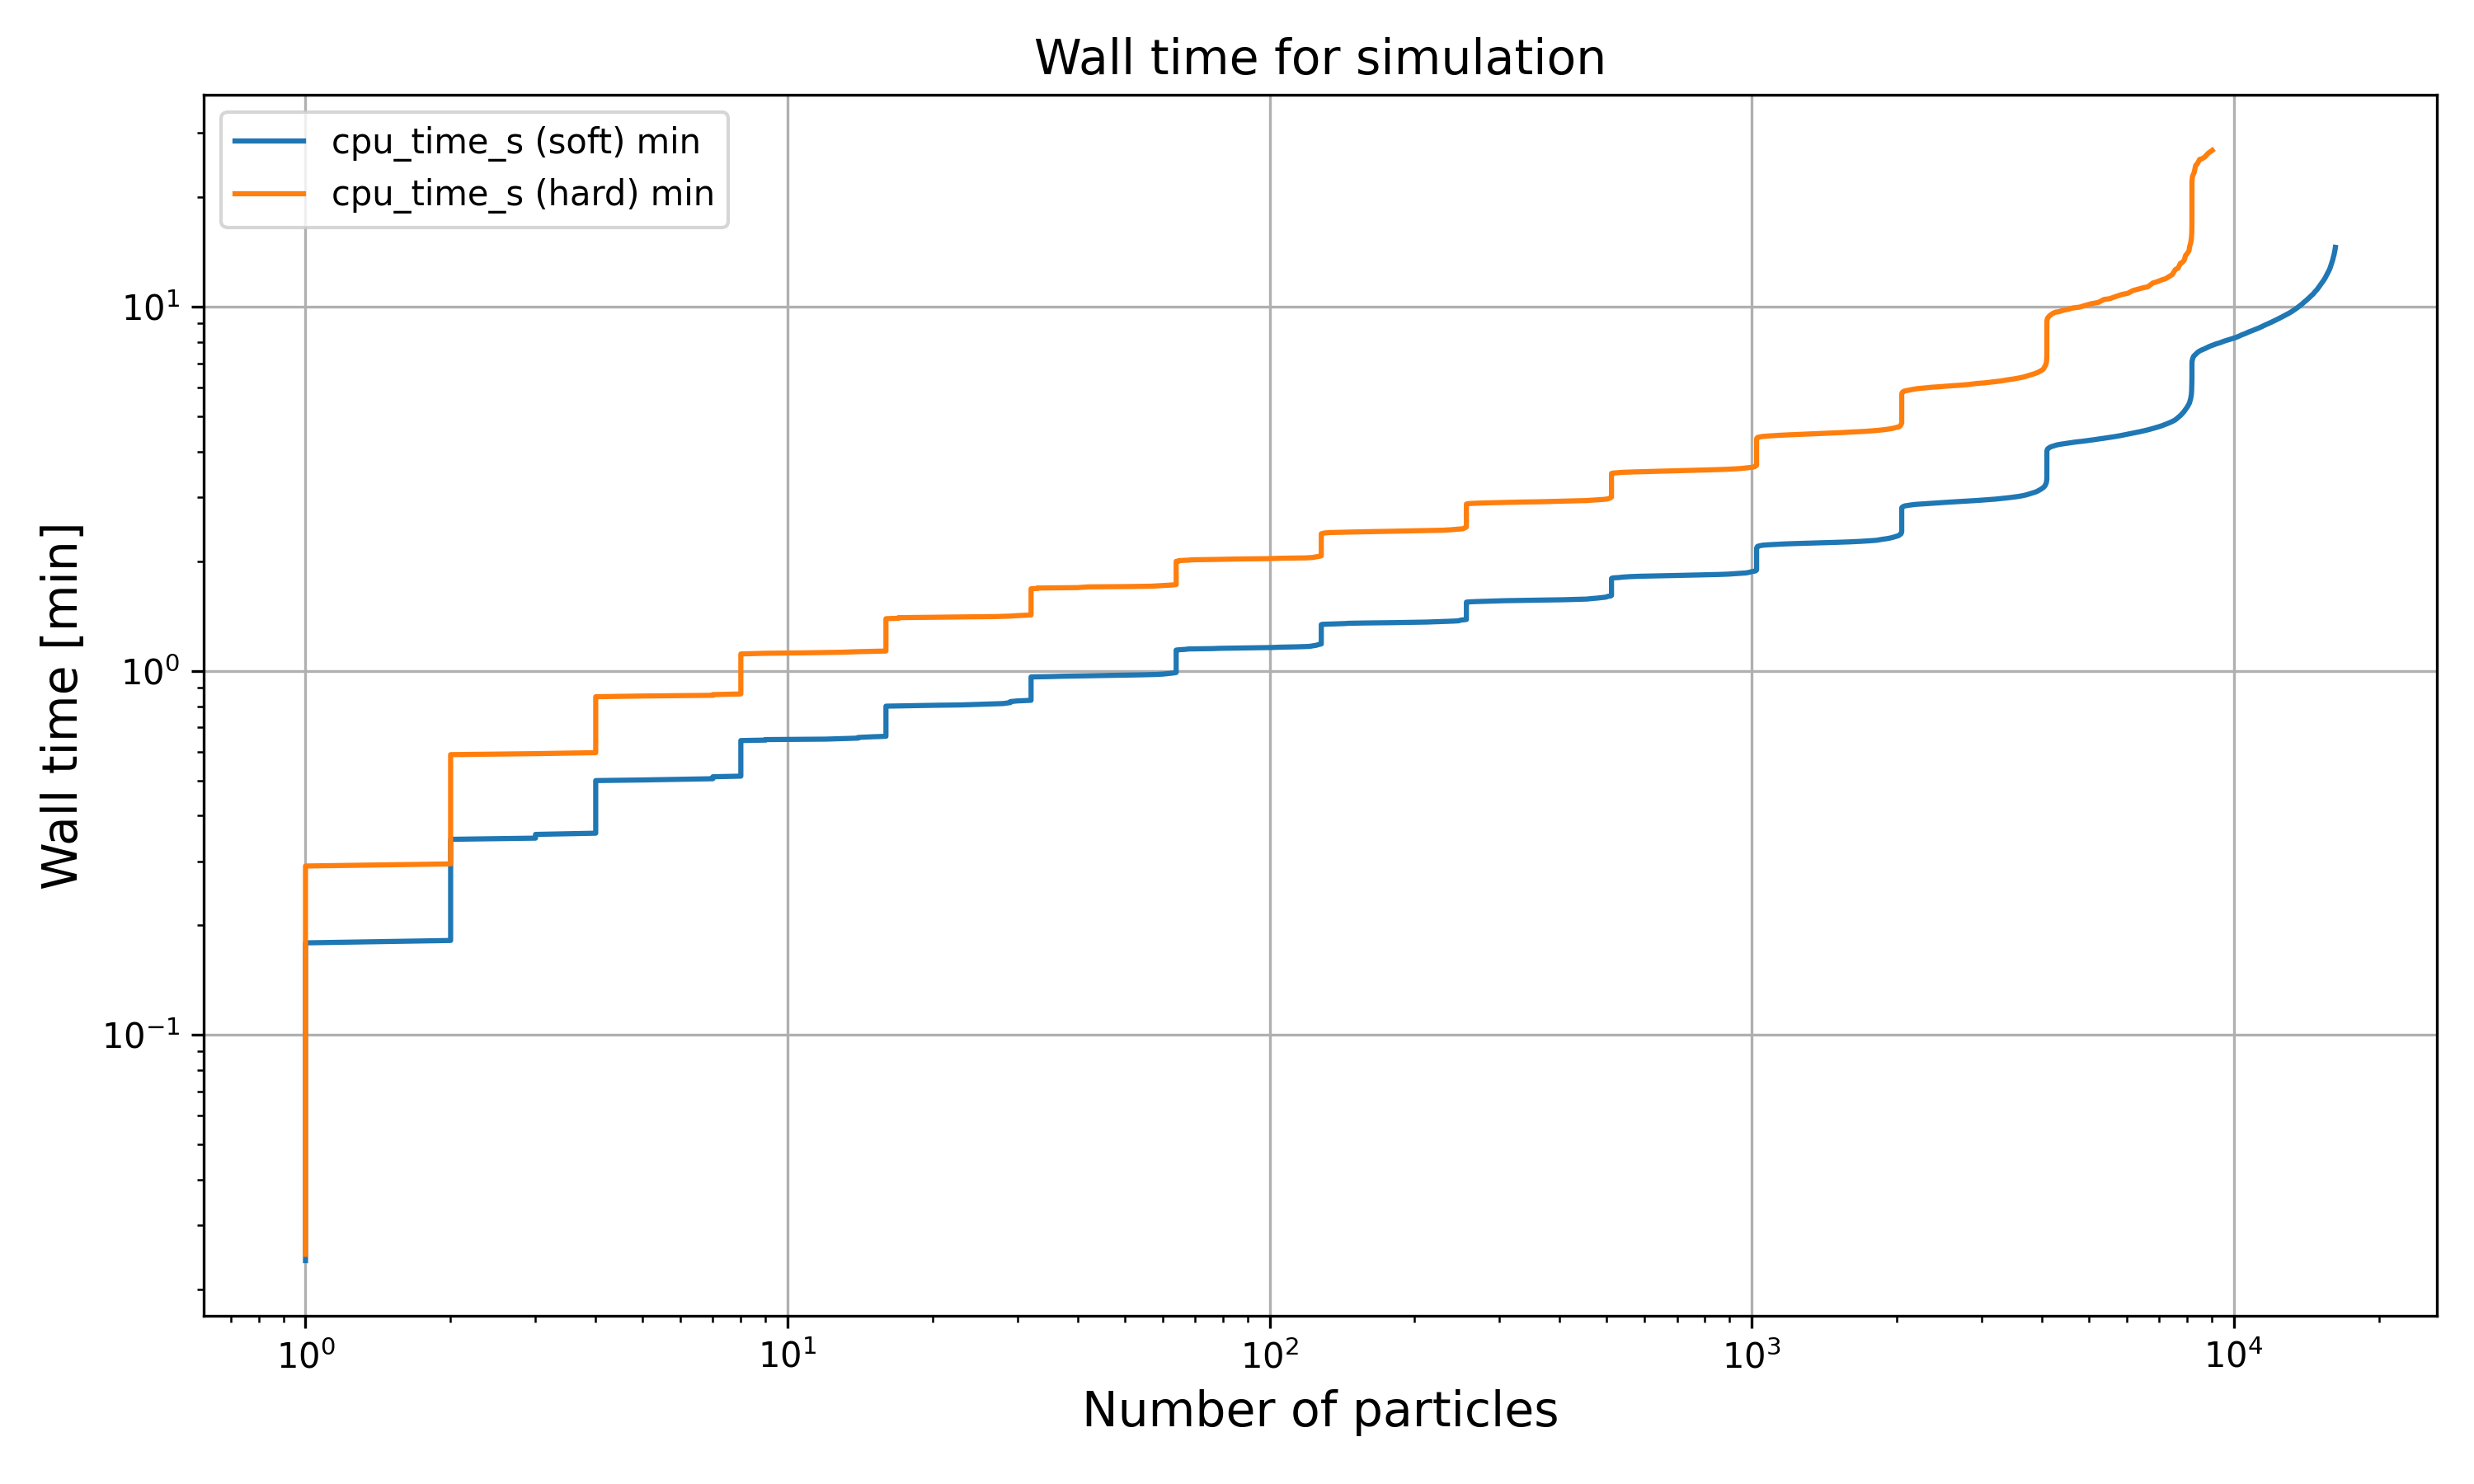
\includegraphics[width=\linewidth]{figures/comparisons/wall_time_simulation.png}
    \caption{Comparison of the total simulation time for the hard and soft collision models over number of particles. The soft model is generally faster by a factor of 1.8.}
    \label{figure:wall_time_simulation}
\end{figure}

\begin{figure}
    \centering
    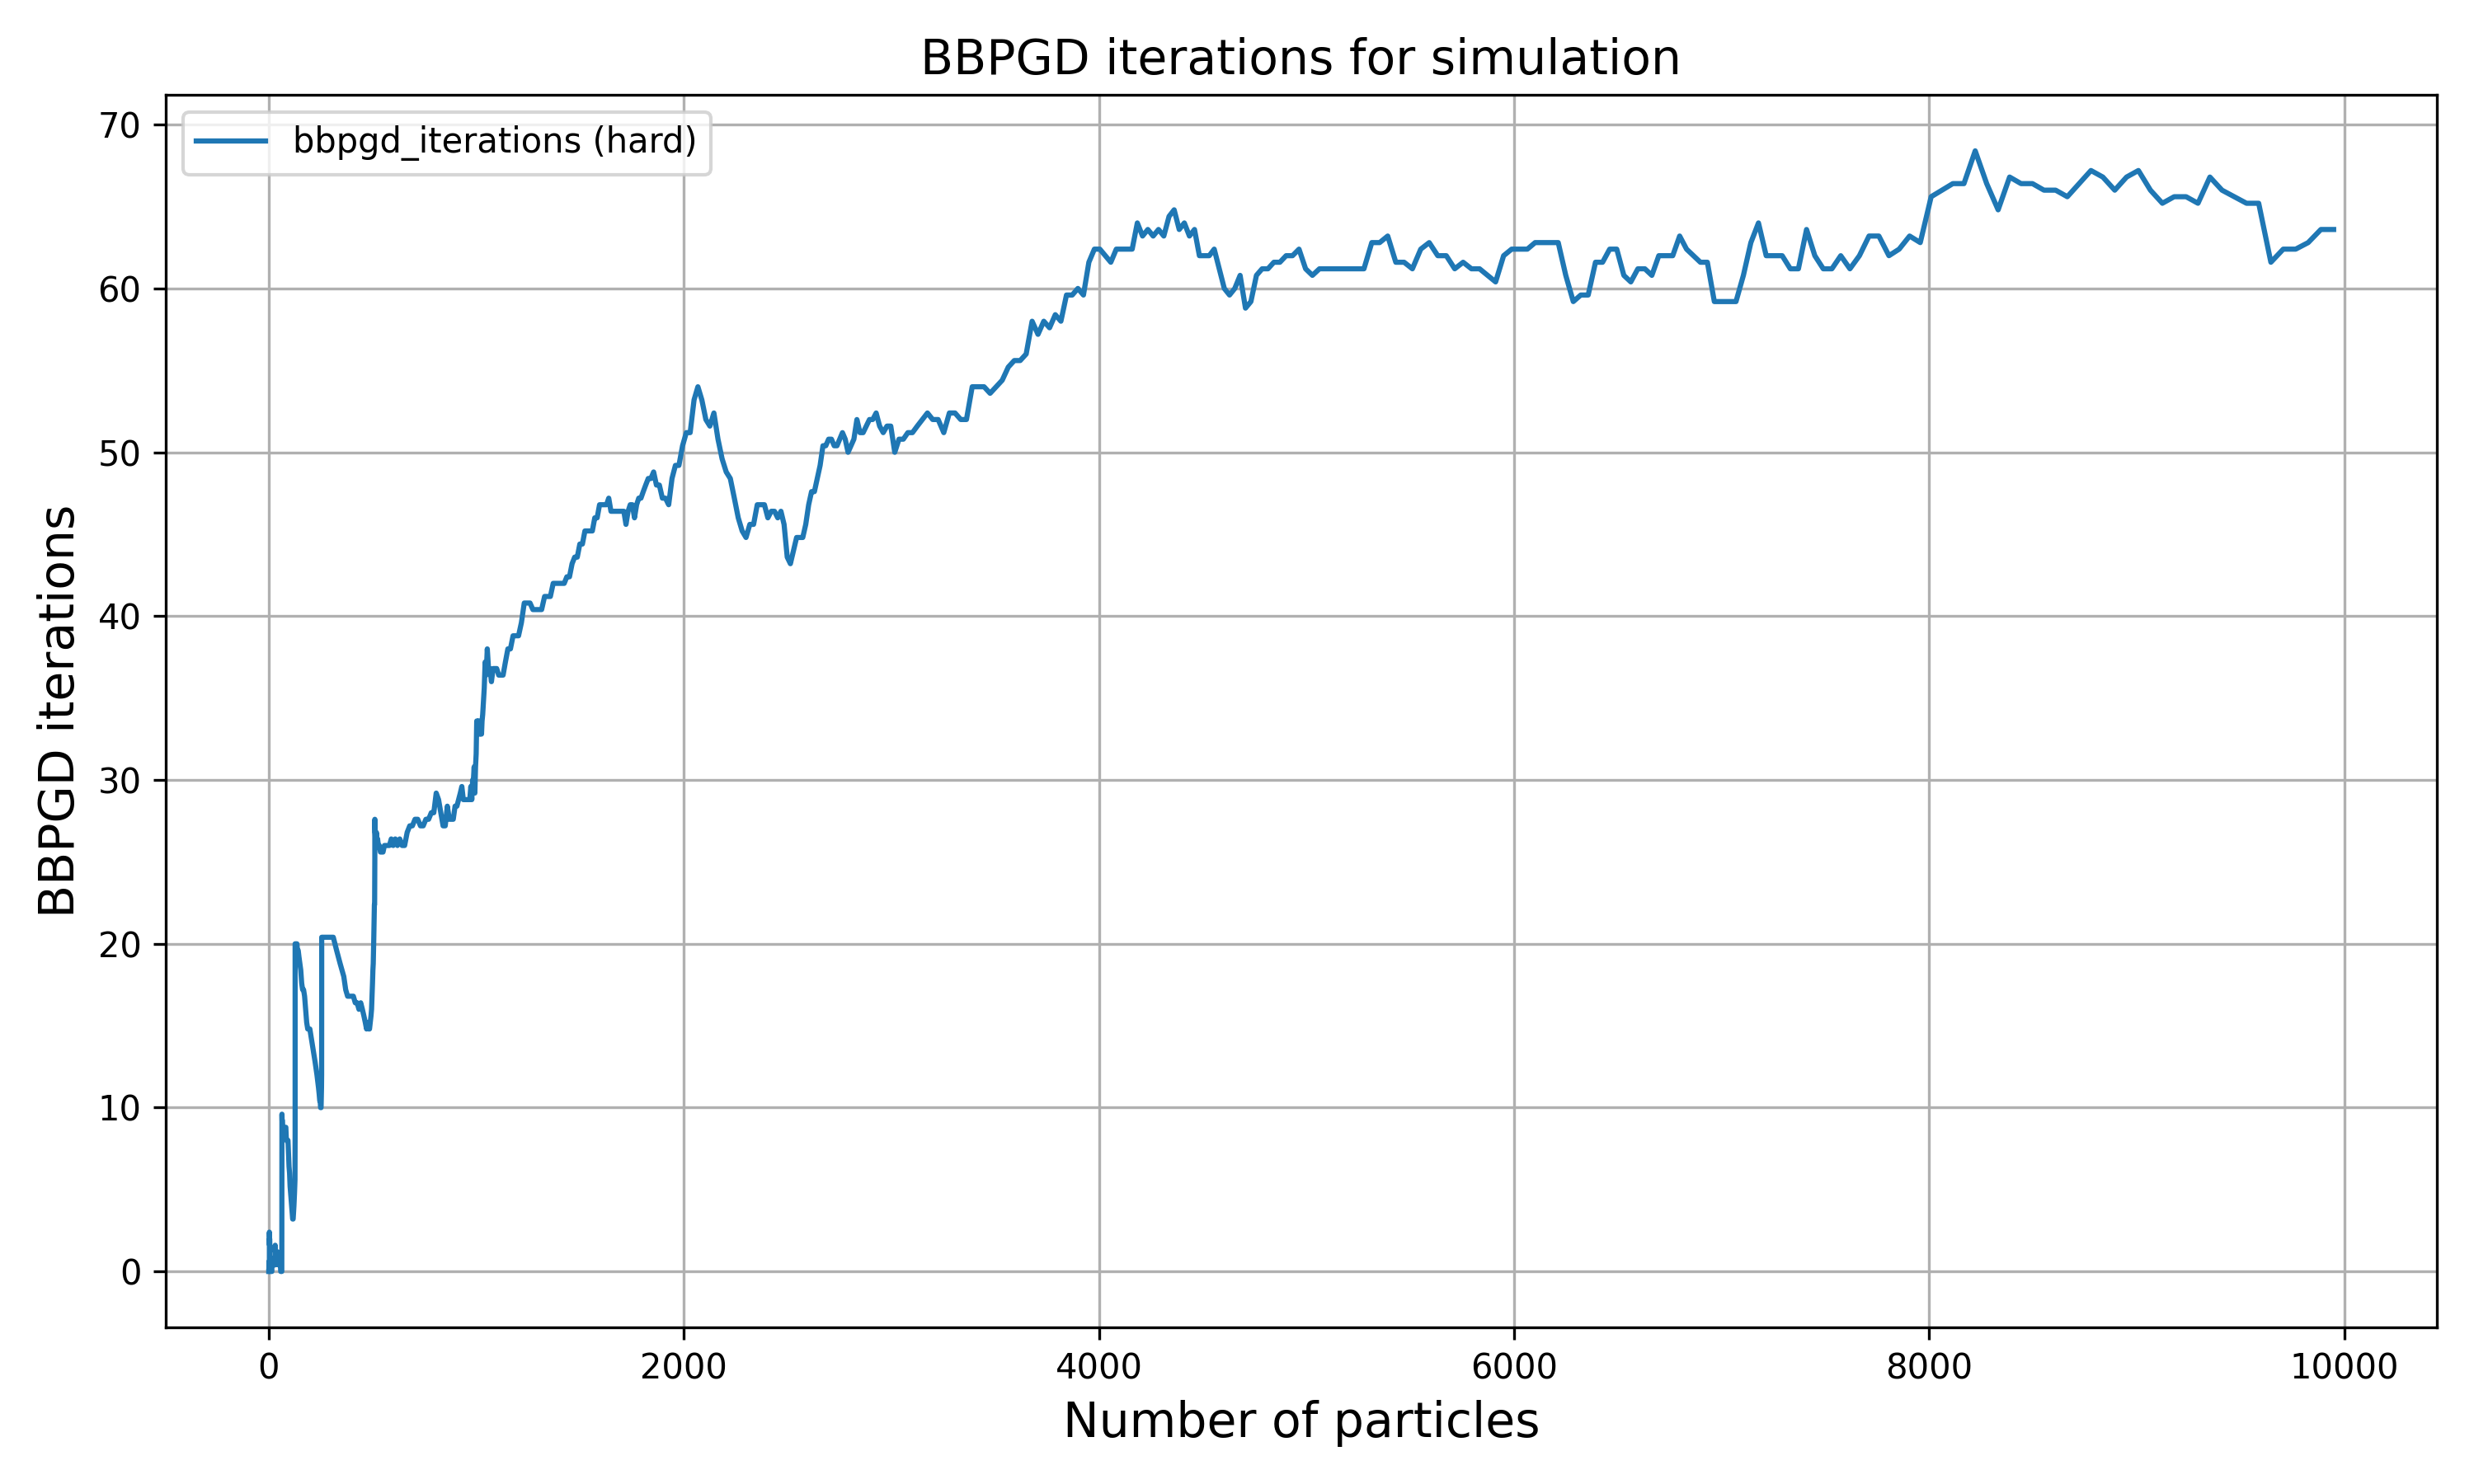
\includegraphics[width=\linewidth]{figures/comparisons/bbpgd_iterations_simulation.png}
    \caption{BBPGD iterations for the hard and soft collision models. To maintain constant particle separation, the hard model needs to solve an LCP iteratively at each time step. The required number of iterations increases with the number of particles.}
    \label{figure:bbpgd_iterations_simulation}
\end{figure}

\newpage
\section{Discussion}
\subsection{Model Selection Insights}


The choice between hard and soft collision models for simulating proliferating cell collectives presents a clear trade-off. The hard model offers precision in enforcing non-overlap but at a considerable computational cost due to LCP solving. The soft model, by employing continuous potentials, offers a potentially much faster simulation pathway, crucially important for exploring large-scale systems or parameter spaces. For many biological pattern formation scenarios, where the precise moment of contact is less critical than the emergent macroscopic behavior, the computational efficiency of the soft model makes it a highly attractive option.

\subsection{Biological Relevance}

Our findings suggest that the simplified mechanics of the soft collision model are sufficient to recapitulate key emergent behaviors like concentric ring formation. This implies that the fundamental drivers of these patterns may be robust to the specific details of collision resolution. The biological plausibility of the soft model lies in its ability to represent continuous pressure and proximity effects between cells, which might be more representative of cellular interactions than instantaneous, purely geometric constraints. The potential for faster simulations with the soft model could enable more extensive exploration of how proliferation rates, cell mechanics, and environmental factors influence colony morphogenesis.

\newpage

\section{Conclusion}

This work demonstrates that a computationally efficient soft collision model can effectively simulate proliferating cell collectives and reproduce complex emergent patterns observed in bacterial colonies, such as concentric rings. While the hard collision model provides exact non-overlap, its computational demands are substantial. The soft collision model offers a compelling alternative, promising significantly improved performance and scalability without a critical loss in qualitative pattern formation fidelity. This makes the soft approach a valuable tool for future large-scale simulations in computational biology and active matter research. Future work will focus on quantitatively detailing these performance benefits and exploring the soft model's behavior under more varied growth and environmental conditions.

\newpage
\tableofcontents


\bibliographystyle{IEEEtran}
\bibliography{literature}

\end{document}